

\documentclass[a4paper,12pt,pdftex,onecolumn]{article}


\addtolength{\textwidth}{3cm}
\addtolength{\evensidemargin}{-1.5cm}
\addtolength{\oddsidemargin}{-1.5cm}

\addtolength{\textheight}{3cm}
\addtolength{\voffset}{-1cm}


%\usepackage{times}
\usepackage{palatino}
%\usepackage{mathpple}


\usepackage{multicol}

\usepackage{amsmath}
\usepackage{amssymb}

\usepackage{dcolumn}

\usepackage{paralist}



\usepackage[utf8]{inputenc}
\usepackage[english]{babel}

\usepackage{graphicx}

\usepackage{xspace}
\newcommand{\etal}{\emph{et al.}\xspace}
\newcommand{\ie}{\emph{i.e.}\xspace}
\newcommand{\eg}{\emph{e.g.}\xspace}
\newcommand{\etc}{\emph{etc.}\xspace}

\usepackage{fancyvrb}
\usepackage{relsize}


\usepackage{fancyhdr} 
\pagestyle{fancy}
% Clear:
\fancyhf{}
% Settings:
\fancyheadoffset{0cm}
\renewcommand{\headrulewidth}{0.5pt} 
\renewcommand{\footrulewidth}{0pt}
% New header style:
\fancyhead[L]{K. O. E. Henriksson}
\fancyhead[C]{Documentation for \textsc{TULIP} 2}
\fancyhead[R]{\thepage}
% New footer style:
% -
% Special case for plain-style pages:
\fancypagestyle{plain}{%
  \fancyhf{}%
  \fancyhead[R]{\thepage}%
}


\usepackage{color}
\definecolor{lightblue}{rgb}{0.7,0.7,1.0}%\def\lightblue{\color{lightblue}}
\definecolor{lightred}{rgb}{1.0,0.85,0.85}
\definecolor{blue}{rgb}{0.0,0.0,1.0}
\definecolor{black}{rgb}{0.0,0.0,0.0}
\definecolor{red}{rgb}{1.0,0.0,0.0}
\definecolor{white}{rgb}{1.0,1.0,1.0}


\usepackage{bm}

\newcommand{\vhat}[1]{{\ifmmode{\widehat{{\bm{\mathrm{#1}}}}} \else $\widehat{\bm{\mathrm{#1}}}$ \fi}}
\newcommand{\vect}[1]{{\ifmmode{{\bm{\mathrm{#1}}}} \else $\bm{\mathrm{#1}}$ \fi}}

\newcommand{\vr}{{\ifmmode{{\bm{\mathrm{r}}}} \else $\bm{\mathrm{r}}$ \fi}}
\newcommand{\vF}{{\ifmmode{{\bm{\mathrm{F}}}} \else $\bm{\mathrm{F}}$ \fi}}



\bibliographystyle{plain}


% Fill in the caption in the braces of the \caption{} command. Put the label
% that you will use with \ref{} command in the braces of the \label{} command.
% Use the figure* environment if the figure should span across the
% entire page. There is no need to do explicit centering.

% \begin{figure}
% \includegraphics{}%
% \caption{\label{}}
% \end{figure}

% \begin{figure}
% \includegraphics{}%
% \caption{\label{}}
% \end{figure}


% Insert the column specifiers (l, r, c, d, etc.) in the empty braces of the
% \begin{tabular}{} command.

% Use the table* environment to get a full-width table in two-column

% \begin{table}%[H] add [H] placement to break table across pages
% \caption{\label{}}
% \begin{ruledtabular}
% \begin{tabular}{}
% Lines of table here ending with \\
% \end{tabular}
% \end{ruledtabular}
% \end{table}



\newcommand{\stars}{\begin{center}%
\vspace{1em plus 0.5em minus 0.5em}%
$\star \qquad \star \qquad \star$%
\vspace{1em plus 0.5em minus 0.5em}%
\end{center}}



\newcommand{\framepar}[1]{
\fbox{
\parbox[t]{0.80\textwidth}{
#1
}}}




%\setlength{\parindent}{0em}
%\setlength{\parskip}{0.75em plus 0.2em minus 0.2em}

\usepackage{parskip}




% End of preamble
\begin{document}



\title{
Documentation for \textsc{TULIP} 2
}
\author{K. Henriksson}
\date{\today}

\maketitle

\begin{abstract}
This \textcolor{black}{booklet} gives an introduction to the \textsc{TULIP}, which is
a program for fitting interatomic potentials to physical data
of different phases and lattices.
\end{abstract}

\tableofcontents






\section{Introduction}

The program \textsc{TULIP} tries to fit a interatomic potential
to \eg given physical properties of compounds \etc. Physical properties are
for instance lattice parameters, cohesive energy, bulk modulus and
elastic constants.

Input is essentially an initial guess for potential parameters,
a list of compounds and their desired properties
(lattice parameters, cohesive energy, mixing energy, bulk modulus,
elastic constants, ...), and technical specifications to guide the fitting.
Using the parametrization, compounds are relaxed in a molecular
dynamics (MD) simulation (MDS), and then the specified physical properties
are calculated.
The fitting routine tries to minimize the merit function. The fitting method
can be selected.




\section{Source code}

0. Prerequisites: Install the \verb+spglib+ package from
\verb+http://spglib.sourceforge.net/+ in a standard location and
remember the location of installed files.

1. Local users only: Download the \verb+libutils+ source code into a folder:

\begin{Verbatim}[fontsize=\relsize{-1},frame=single]
git clone /home/phys-data/people/koehenri/repos/libutils.git
\end{Verbatim}

The \verb+libutils+ directory will be created. Descend into it and
follow the instructions in the Readme file to make and install the
library.

2. Local users only: Download the \verb+tulip2+ source code into a folder:

\begin{Verbatim}[fontsize=\relsize{-1},frame=single]
git clone /home/phys-data/people/koehenri/repos/tulip2.git
\end{Verbatim}

The \verb+tulip2+ directory will be created. Descend into it and
follow the instructions in the Readme file to make and install the
fitting code.

3. The static version \verb+tulip_static+ can be copied to other
computer systems having the same architecture and be run there
without any additional effort. The shared library version requires
adding the \verb+libutils+ library to the library path.

\stars

To download updated versions of these codes descend into the root
directories (e.g. \verb+tulip2+) and execute

\begin{Verbatim}[fontsize=\relsize{-1},frame=single]
git pull
\end{Verbatim}

This will fetch and merge updated code with your local copy.

\stars

The \verb+tulip2/examples+ directory contains some ready-made examples,
which can be run without additional editing to get a better feel
for how the code works.




\section{Program arguments}

\begin{Verbatim}[fontsize=\relsize{-3},frame=single]
TULIP version 2 (c) Krister Henriksson 2013-
Purpose: Fit data to an interatomic potential.
Usage:
     tulip arguments [options]
Arguments:
     -pf file           Path to file containing potential information.
     -gf file           Path to file containing geometry information.

Options:
     -sf file           Path to file containing technical specifications about the calculations.
     -ro                Only calculate properties of reference compounds, then exit. Default: not used.
     -nof               Only calculate properties of reference and read-in compounds, then exit. Default: not used.
     -xyz               Use traditional XYZ format when writing XYZ files. Default: not used.
                        The extended XYZ format (http://jrkermode.co.uk/quippy/io.html#extendedxyz)
                        is used by default.

     -dfitpropn         Show information about fitting of properties. Here 'n' must be
                        an integer. Supported: 0-4. 0: debug fitting method. 1-4: debug deeper.
                        lying methods used by the fitting method. Default: not used
                        NOTE: 0 also shows some info about the initial Chi^2 object.
     -dfitpotn          Show information about fitting of potentials. Here 'n' have a similar
                        role as for fitting of the properties.
                        NOTE 1: 0 also shows some info about the initial Chi^2 object.
                        NOTE 2: 'fitpot0' is always set to true, others are false by default.

     -dforces           Debug the forces. Default: not used
     -dpressure         Debug the pressure. Default: not used
     -dmdsprop          Debug MDS runs of the structures. Default: not used
     -dall              Activate all debugging options (top level only). Default: not used

     -mif               Suggest an initial fit and exit. Default: not used

     -omp               Request maximal number of threads (8) for any OpenMP parts.
     -omp_nt num        Request 'num' number of threads for any OpenMP parts. Default: 1
\end{Verbatim}


Main arguments:

\begin{Verbatim}[fontsize=\relsize{-1},frame=single]
-pf potinfofile     This file contains info about the elements and interactions.
-gf geominfofile    This file contains the info about the compounds which are
                    to be fitted.
\end{Verbatim}

Recommended options to always use:

\begin{Verbatim}[fontsize=\relsize{-1},frame=single]
-sf specsinfofile   This file contains settings steering the calculation of
                    properties of read-in compounds and the fitting process.
\end{Verbatim}

Useful options:

\begin{Verbatim}[fontsize=\relsize{-1},frame=single]
-ro            Calculate properties of reference (single-species) compounds
               and quit.
-nof           Calculate properties of reference and read-in compounds and quit.
               This is useful when parametrization is finalized and high-accuracy
               values of properties are desired (use long MD relaxation times!).
-mif           Obtain an initial partial fit to start from.
-dmdsprop      Show progress of all MD relaxations of all compounds.
\end{Verbatim}

Note: The OpenMP options can be used, but the OpenMP parallellization has not been
extensively debugged. Some cache trashing is likely to occur, degrading performance.






\section{Potentials}

In \textsc{TULIP} the following potentials are subject to fitting:
(i)  the ABOP (Analytical Bond Order Potential).
The EAM (Embedded Atom Method) potential is understood by the
program, but this type of interactions cannot be fitted.






\subsection{ABOP potential}

The Brenner-Tersoff or ABOP potential gives the total energy of a system of atoms as

\begin{equation}
V = {1 \over 2} \sum_i \sum_{j} f_{c,ij} \left( V_{R,ij} - B_{ij} V_{A,ij} \right)
= \sum_i \sum_{j>i} f_{c,ij} \left( V_{R,ij} - \overline{B}_{ij} V_{A,ij} \right),
\label{eq:abop}
\end{equation}

Here

\begin{equation}
\overline{B}_{ij} = {B_{ij} + B_{ji} \over 2}
\end{equation}

Note:

\begin{equation}
V_{ij} \equiv  f_{c,ij} \left( V_{R,ij} - B_{ij} V_{A,ij} \right)
\end{equation}

may not be equal to $V_{ji}$.

The repulsive ($R$) and attractive ($A$) parts are

\begin{eqnarray}
  V_{R,ij} = {D_0 \over S-1} \exp\left[ - \beta \sqrt{2S} (r_{ij} -r_{0,ij})
  \right] \\
  V_{A,ij} = {S D_0 \over S-1} \exp\left[ - \beta \sqrt{2/S} (r_{ij} -r_{0,ij})
  \right]
\end{eqnarray}

with

\begin{equation}
r_{ij} = |\mathbf{r}_{ij}| = | \mathbf{r}_i - \mathbf{r}_j |
\end{equation}

The cutoff-function is

\begin{equation}
f_c(r) =
\left\{
\begin{array}{ll}
1,                   & r \leq R - D, \\
{1 \over 2} \left( 1 - \sin \left( {\pi \over 2} {r - R \over D}
    \right) \right), & R-D < r < R + D \\
0,                   & r \geq R + D
\end{array}
\right.
\end{equation}

Hence, full interaction is felt when $r<R-D$, and no interaction when $r>R+D$,
making the cutoff distance $r_c = R+D$. The derivative is

\begin{equation}
f'_{c}(r) =
\left\{
\begin{array}{ll}
0,                   & r \leq R - D, \\
{1 \over 2} \left( 1 - {\pi \over 2D} \cos \left( {\pi \over 2} {r - R \over D}
    \right) \right), & R-D < r < R + D \\
0,                   & r \geq R + D
\end{array}
\right.
\end{equation}




The bond-order parameter is defined as

\begin{equation}
B_{ij} = \left( 1 + \chi_{ij} \right)^{-p_{ij}}
\end{equation}

The usual ABOP has $p_{ij} \equiv 1/2$.

Here

\begin{equation}
\chi_{ij} =
\sum_{k, k \neq i, k \neq j} f_{c,ik} g_{ijk}(\theta_{ijk})
\omega_{ijk} \exp\left[ \alpha_{ijk}(r_{ij} - r_{ik}) \right]
\end{equation}

We have now three different possibilities:

(V1) $\alpha_{ijk}$ and $\omega_{ijk}$ are used as parameters.

(V2) If $\alpha_{ijk}$ is used but $\omega_{ijk}$ is not, then the
Brenner form is used for the latter:

\begin{equation}
\omega_{ijk} = \exp\left[
- \alpha_{ijk} ( r_{0,ij} - r_{0,ik})
\right]
\label{eq:omegaijk}
\end{equation}

and $\omega_{ijk}$ is \textbf{not} a separate parameter.

(V3) If $\alpha_{ijk}$ is not used and $2\mu_{ik}$ is used, then the
whole factor

\begin{equation}
\omega_{ijk} \exp\left[ \alpha_{ijk}(r_{ij} - r_{ik}) \right]
\end{equation}

is replaced in its entirety by

\begin{equation}
\exp\left[ 2\mu_{ik} (r_{ij} - r_{ik}) \right]
\end{equation}

The function $g_{ijk}(\theta_{ijk})$ is given by the expression

\begin{equation}
g_{ijk}(\theta_{ijk}) = \gamma \left(
1 + {c^2 \over d^2} - {c^2 \over d^2 + (h + \cos \theta_{ijk})^2}
\right)
\end{equation}

where $\theta_{ijk}$ is the angle between the bonds $ij$ and $ik$.

The ABOP potential is insufficient for small interatomic distances.
To ensure a more correct description a (repulsive) potential
$V_{\mathrm{rep}}(r)$ --- e.g. the ZBL potential --- describing
interactions at small distances should be used.
The original potential presented above is then modified to

\begin{equation}
V(r) = (1-F(r)) V_{\mathrm{rep}}(r) + F(r) V_{\mathrm{orig}}(r)
\end{equation}

where $F(r)$ is the Fermi function

\begin{equation}
F(r) = 1/(1 + e^{-b_f(r-r_f)})
\end{equation}

and $b_f, r_f$ are parameters that need to be supplied.

All parameters that can be used with the ABOP potential are:

\begin{center}
\begin{tabular}{|l|l|}
\hline
\hline
Parameter & Notes \\
\hline
\hline
$D_0$ & \\
$r_0$ & \\
$\beta$ & \\
$S$ & \\
$\gamma$ & \\
$c$ & \\
$d$ & \\
$h$ & \\
$D$ & \\
$R$ & Cutoff is $r_c = R + D$. \\
$b_f$ & Defaults to $10$. \\
$r_f$ & Defaults to $1$. \\
$p$ & Defaults to $1/2$. \\
\hline
(V1) $\alpha_{ijk}$ and $\omega_{ijk}$ & \\
(V2) $\alpha_{ijk}$ & $\omega_{ijk}$ given by Eq.~(\ref{eq:omegaijk}).\\
(V3) $2\mu_{ik}$ & \\
\hline
\hline
\end{tabular}
\end{center}





\subsection{EAM potentials}

EAM potentials can as of now not be fitted, but only be used
as read-in potentials.

The total energy of a solid is in the EAM formalism

\begin{equation}
V = {1 \over 2} \sum_i \sum_{j, j \neq i} V_2(r_{ij})
+ \sum_i a_s F_s(\rho^a_{s,i})
+ \sum_i a_p F_p(\rho^a_{p,i})
+ \sum_i a_d F_d(\rho^a_{d,i}).
\end{equation}

Here $a_i$ is 1 if the band $i$ is included, else it is 0.
Also,

\begin{equation}
\rho^a_i = \sum_{j=1, j\neq i} \rho(r_{ij}),
\end{equation}

where $\rho(r)$ is the atomic electron density at distance $r$
from an atom. The program recognized the EAM versions displayed
in table~\ref{tab:kw-eam}.

\stars



The EAM potentials are read in from files. The format of these
is shown in tables~\ref{tab:kw-eam-ff}-\ref{tab:kw-eam-ff3}.

\stars

{\large \textit{\textbf{Note:}}} The \verb+Nr+ points $(r, V_2)$
in the EAM files are read in as
$r = 0, \ldots,($\verb+Nr+$-1)$\verb+dr+.
To avoid any problems, we must have \verb+Nr+ $\times$ \verb+dr+ $>$ \verb+rcut+.
For instance, use 
\verb+Nr+ $\times$ \verb+dr+ $=$ \verb+rcut+ $+ 10 \times$ \verb+dr+.



\begin{table}[!h]
\caption{
Recognized EAM flavors.
\label{tab:kw-eam}
}
\begin{center}
\begin{tabular}{|l|l|}
\hline
\hline
\verb+EAM-s+         & EAM with only $s$ embedding energy \\
\verb+EAM-p+         & EAM with only $p$ embedding energy \\
\verb+EAM-d+         & EAM with only $d$ embedding energy \\
\verb+EAM-sp+        & EAM with $s$ and $p$ embedding energies \\
\verb+EAM-sd+        & EAM with $s$ and $d$ embedding energies \\
\verb+EAM-spd+       & EAM with $s$, $p$, and $d$ embedding energies \\
\hline
\hline
\end{tabular}
\end{center}
\end{table}


\begin{table}[!h]
\caption{
EAM file format when a single embedding energy is used.
Note: First and second lines are ignored.
\label{tab:kw-eam-ff}
}
\begin{center}
\begin{tabular}{|l|}
\hline
\hline
\verb+Comment line+ \\
\verb+Z1 Z2 mass1 mass2 latpar1 latpar2 latname1 latname2+ \\
\verb+Nrho drho Nr dr rcut+ \\
(Nrhod points of $F_s$ or $F_p$ or $F_d$ ) \\
(Nr points of $V_2$)  \\
(Nr points of $\rho_s$ or $\rho_p$ or $\rho_d$ ) \\
\hline
\hline
\end{tabular}
\end{center}
\end{table}

\begin{table}[!h]
\caption{
EAM file format when two embedding energies are used.
Example is for $s$ and $d$ embedding energies.
Note: First and second lines are ignored.
\label{tab:kw-eam-ff2}
}
\begin{center}
\begin{tabular}{|l|}
\hline
\hline
\verb+Comment line+ \\
\verb+Z1 Z2 mass1 mass2 latpar1 latpar2 latname1 latname2+ \\
\verb+Nrhod drhod Nr dr rcut Nrhos drhos+ \\
(Nrhod points of $F_d$) \\
(Nr points of $V_2$)  \\
(Nr points of $\rho_d$) \\
(Nrhos points of $F_s$) \\
(Nr points of $\rho_s$) \\
\hline
\hline
\end{tabular}
\end{center}
\end{table}


\begin{table}[!h]
\caption{
EAM file format when three embedding energies are used.
Note: First and second lines are ignored.
\label{tab:kw-eam-ff3}
}
\begin{center}
\begin{tabular}{|l|}
\hline
\hline
\verb+Comment line+ \\
\verb+Z1 Z2 mass1 mass2 latpar1 latpar2 latname1 latname2+ \\
\verb+Nrhod drhod Nr dr rcut Nrhos drhos Nrhop drhop+ \\
(Nrhod points of $F_d$) \\
(Nr points of $V_2$) \\
(Nr points of $\rho_d$) \\
(Nrhos points of $F_s$) \\
(Nr points of $\rho_s$) \\
(Nrhop points of $F_p$) \\
(Nr points of $\rho_p$) \\
\hline
\hline
\end{tabular}
\end{center}
\end{table}








\section{Read-in files}


All specifications about the fitting procedure, physical properties,
and calculations in general are given in read-in files:
(i) file containing settings for the potentials,
(ii) file containing physical properties, and
(iii) file containing technical specifications about the
calculations. The last file is optional.

The delimiters separating tokens in the read-in files are:
tabulator, space, and the following characters: \verb+:,()[]=+. The
point is not a delimiter. Character strings which are not part of the
input value for an option are simply ignored.





\subsection{File: Elements and interactions information}


An overview of which potentials that can be read in from tabulated data
in $(x, y)$ format and those which can be specified via parameters only
is shown in Table~\ref{tab:pot-da}.


\begin{table}[!h]
\caption{
R = Can be read in from data file.
A = Can be specified by parameters.
\label{tab:pot-da}
}
\begin{center}
\begin{tabular}{|l|l|l|}
\hline
\hline
Potential   & R    & A  \\
\hline
EAM-*       & Yes  & No \\
ABOP        & No   & Yes \\
\hline
\hline
\end{tabular}
\end{center}
\end{table}

\stars


Complete example:


\begin{Verbatim}[fontsize=\relsize{-1},frame=single]

# MUST BE FIRST:
# Number of elements:
nelem = 3

# MUST BE SECOND:
# Element names:
elem(1) = Fe
elem(2) = Cr
elem(3) = C


# Optional:
atomtype(Fe) = 1
atomtype(Cr) = 2
atomtype(C)  = 3


# Masses
mass(Fe) = 55.8470
mass(Cr) = 51.9961
mass(C ) = 12.0110


# Reference lattices:
lat(Cr, Cr) = skip   BCC  Calc. for this will be skipped, we will have Ecoh(Cr)=0.0.
lat(Fe, Fe) = BCC
lat(C,  C ) = GRA

# Supported ref. lattices:
# DIM1 (homomer), DIM2 (heteromer), SC, BCC, BCC-P, FCC, FCC-P,
# DIA, HCP, GRA, GRP (graphene)
# The ...-P versions refer to alternate structures with
# non-Cartesian primitive vectors.

a(Cr, Cr)  = 2.87
a(Fe, Fe)  = 2.87
#########################################################################
# Use accurate values for C, otherwise the graphite might explode due
# to massive pressure!!! Also, use small enough time step!!!
#########################################################################
a(C,  C )   = 1.46   rNN for graphite (GRA)      DIA: 3.55647765821
c(C,  C )   = 6.689
# Also possible:
# bpa(C, C) = ...
# cpa(C, C) = ...


# Interaction types:
iac(Fe, Fe) = ABOP
iac(Cr, Cr) = ABOP
iac(C,  C ) = ABOP
iac(Fe, Cr) = ABOP   symmetric
iac(Fe, C ) = ABOP   symmetric
iac(Cr, C ) = ABOP   symmetric


# Fit this interaction? The interaction must be analytical.
fit(Fe, Cr) = yes    symmetric


# Repulsive potentials (ZBL):

use_rep_core( Fe, Fe ) = yes
use_rep_core( Cr, Cr ) = yes
use_rep_core( C,  C  ) = yes
use_rep_core( Fe, Cr ) = yes
use_rep_core( Fe, C  ) = yes
use_rep_core( Cr, C  ) = yes

# Parameters for fixed interactions

potpar( Fe, Fe ):D0 = 1.5
potpar( Fe, Fe ):r0 = 2.29
potpar( Fe, Fe ):beta = 1.4
potpar( Fe, Fe ):S = 2.0693109
potpar( Fe, Fe ):gamma = 0.0115751
potpar( Fe, Fe ):c = 1.2898716
potpar( Fe, Fe ):d = 0.3413219
potpar( Fe, Fe ):h = -0.26
potpar( Fe, Fe ):R = 3.15
potpar( Fe, Fe ):D = 0.2
potpar( Fe, Fe ):bfermi = 10
potpar( Fe, Fe ):rfermi = 1

potpar(Cr, Cr ):D0 = 4.04222081
potpar(Cr, Cr ):r0 = 2.13018547
potpar(Cr, Cr ):beta = 1.62158721
potpar(Cr, Cr ):S = 3.36793914
potpar(Cr, Cr ):gamma = 0.02388562
potpar(Cr, Cr ):c = 1.03288255
potpar(Cr, Cr ):d = 0.13813230
potpar(Cr, Cr ):h = -0.28569237
potpar(Cr, Cr ):R = 3.2
potpar(Cr, Cr ):D = 0.20
potpar( Cr, Cr ):bfermi = 12
potpar( Cr, Cr ):rfermi = 1.7

potpar(C, C ):D0 = 6.0
potpar(C, C ):r0 = 1.39
potpar(C, C ):beta = 2.1
potpar(C, C ):S = 1.22
potpar(C, C ):gamma = 2.0813e-4
potpar(C, C ):c = 330.0
potpar(C, C ):d = 3.5
potpar(C, C ):h = 1.0
potpar(C, C ):R = 1.85
potpar(C, C ):D = 0.15
potpar( C , C  ):bfermi = 8
potpar( C , C  ):rfermi = 0.6

potpar(Fe, C ):D0 = 3.95000634
potpar(Fe, C ):r0 = 1.53426579
potpar(Fe, C ):beta = 1.82109816
potpar(Fe, C ):S = 1.43035110
potpar(Fe, C ):gamma = 0.07485571
potpar(Fe, C ):c = 1.11674155
potpar(Fe, C ):d = 0.94663188
potpar(Fe, C ):h = -0.18665305
potpar(Fe, C ):R = 2.6
potpar(Fe, C ):D = 0.20
potpar( Fe, C  ):bfermi = 10
potpar( Fe, C  ):rfermi = 1

potpar( Cr, C ):D0        =  2.77620074
potpar( Cr, C ):r0        =  1.81289285
potpar( Cr, C ):beta      =  2.00816371
potpar( Cr, C ):S         =  2.04637644
potpar( Cr, C ):gamma     =  0.00068830
potpar( Cr, C ):c         =  3.93353757
potpar( Cr, C ):d         =  0.17497204
potpar( Cr, C ):h         =  -0.17850001
potpar( Cr, C ):R         =  2.95
potpar( Cr, C ):D         =  0.1
potpar( Cr, C  ):bfermi = 8
potpar( Cr, C  ):rfermi = 1.2


# Parameters for fittable interactions

     potpar( Fe, Cr ):D0 = 3.48049488
min: potpar( Fe, Cr ):D0 = 0.1
max: potpar( Fe, Cr ):D0 = 10.0

     potpar( Fe, Cr ):r0 = 2.16998952
min: potpar( Fe, Cr ):r0 = 1.0
max: potpar( Fe, Cr ):r0 = 5.0

     potpar( Fe, Cr ):beta = 1.75467567
min: potpar( Fe, Cr ):beta = 1.0
max: potpar( Fe, Cr ):beta = 5.0

     potpar( Fe, Cr ):S  = 2.28661503
min: potpar( Fe, Cr ):S  = 1.1
max: potpar( Fe, Cr ):S  = 5.0

     potpar( Fe, Cr ):gamma = 0.15766130
min: potpar( Fe, Cr ):gamma = 1e-5
max: potpar( Fe, Cr ):gamma = 1e5

     potpar( Fe, Cr ):c = 0.48531613
min: potpar( Fe, Cr ):c = -1e5
max: potpar( Fe, Cr ):c =  1e5

     potpar( Fe, Cr ):d  = 0.31427413
min: potpar( Fe, Cr ):d  =  -1e5
max: potpar( Fe, Cr ):d  =   1e5

     potpar( Fe, Cr ):h  = -0.69
min: potpar( Fe, Cr ):h  =  1.0
max: potpar( Fe, Cr ):h  =  1.0

     potpar( Fe, Cr ):R  = 3.10
min: potpar( Fe, Cr ):R  = 2.0
max: potpar( Fe, Cr ):R  = 2.0

     potpar( Fe, Cr ):D         = 0.15
min: potpar( Fe, Cr ):D  = 1.0
max: potpar( Fe, Cr ):D  = 1.0

     potpar( Fe, Cr ):bfermi = 10
min: potpar( Fe, Cr ):bfermi =  5
max: potpar( Fe, Cr ):bfermi = 15

     potpar( Fe, Cr ):rfermi = 1
min: potpar( Fe, Cr ):rfermi = 0.1
max: potpar( Fe, Cr ):rfermi = 5



# ABOP alpha and omega parameters

################################################################
##
##  NOTE: There are NO ABOP alpha, omega, 2mu parameters used by default.
##        Only the specified ones are used.
##        Defaults: alpha=2mu=0.0 and omega=1.0 as constants.
##
##        If an omega parameter is specified it is taken as an
##        independent parameter (non-Brenner form), otherwise
##        it is constructed from alpha parameters --- if they are
##        specified --- as
##
##          "omega_ijk" = exp( alpha_ijk*(r0_ij - r0_ik) )
##
################################################################


# Fixed:

abop_alpha( Fe, Fe, Fe ) = 0.0
abop_omega( Fe, Fe, Fe ) = 1.0

abop_alpha( Cr, Cr, Cr ) = 1.39662066
abop_omega( Cr, Cr, Cr ) = 1.0

abop_alpha( C, C, C ) = 0.0
abop_omega( C, C, C ) = 1.0

abop_alpha( Cr, Cr, C  )        = 0.8640643600
abop_alpha( Cr, C , Cr )        = -1.7520448300
abop_alpha( C, Cr, Cr )        = 0.6122158900
abop_alpha( C, C , Cr )        = 0
abop_alpha( C, Cr, C )        = 0
abop_alpha( Cr, C, C  )        = 0

abop_omega( Cr, Cr, C  )        = 1.6402877600
abop_omega( Cr, C , Cr )        = 0.2939996300
abop_omega( C, Cr, Cr )        = 0.4190507900
abop_omega( C, C , Cr )        = 1
abop_omega( C, Cr, C )        = 1
abop_omega( Cr, C, C  )        = 1



# Fittable:

     abop_alpha( Fe, Fe, Cr ) = 1.0
min: abop_alpha( Fe, Fe, Cr ) =  100.0
max: abop_alpha( Fe, Fe, Cr ) =  100.0

     abop_alpha( Fe, Cr, Fe ) = 1.0
min: abop_alpha( Fe, Cr, Fe ) =  100.0
max: abop_alpha( Fe, Cr, Fe ) =  100.0

     abop_alpha( Cr, Fe, Fe ) = 1.0
min: abop_alpha( Cr, Fe, Fe ) =  100.0
max: abop_alpha( Cr, Fe, Fe ) =  100.0

     abop_alpha( Cr, Fe, Cr ) = 1.0
min: abop_alpha( Cr, Fe, Cr ) =  100.0
max: abop_alpha( Cr, Fe, Cr ) =  100.0

     abop_alpha( Fe, Cr, Cr ) = 1.0
min: abop_alpha( Fe, Cr, Cr ) =  100.0
max: abop_alpha( Fe, Cr, Cr ) =  100.0

     abop_alpha( Cr, Cr, Fe ) = 1.0
min: abop_alpha( Cr, Cr, Fe ) =  100.0
max: abop_alpha( Cr, Cr, Fe ) =  100.0




     abop_omega( Fe, Fe, Cr ) = 1.0
min: abop_omega( Fe, Fe, Cr ) =  100.0
max: abop_omega( Fe, Fe, Cr ) =  100.0

     abop_omega( Fe, Cr, Fe ) = 1.0
min: abop_omega( Fe, Cr, Fe ) =  100.0
max: abop_omega( Fe, Cr, Fe ) =  100.0

     abop_omega( Cr, Fe, Fe ) = 1.0
min: abop_omega( Cr, Fe, Fe ) =  100.0
max: abop_omega( Cr, Fe, Fe ) =  100.0

     abop_omega( Cr, Fe, Cr ) = 1.0
min: abop_omega( Cr, Fe, Cr ) =  100.0
max: abop_omega( Cr, Fe, Cr ) =  100.0

     abop_omega( Fe, Cr, Cr ) = 1.0
min: abop_omega( Fe, Cr, Cr ) =  100.0
max: abop_omega( Fe, Cr, Cr ) =  100.0

     abop_omega( Cr, Cr, Fe ) = 1.0
min: abop_omega( Cr, Cr, Fe ) =  100.0
max: abop_omega( Cr, Cr, Fe ) =  100.0


# Not used:
#     abop_2mu( Fe, Cr ) = 1.0
#     abop_2mu( Cr, Fe ) = 1.0


\end{Verbatim}








\subsection{File: Compounds information}

In order to specify a physical property to be fitted,
the keywords in example below must be used.

Keywords are grouped into sets than begin with the string
LAT on a separate line. Properties in each set refer to
the same structure/lattice/geometry.

\textbf{All properties that are specified (=set) are activated as fitting
targets.}


Complete listing of options for a lattice: Note that \verb+...+ means that
numerical values (single or severeal ones) are expected, and \verb+***+ means
that a string is needed.


\begin{Verbatim}[fontsize=\relsize{-1},frame=single]

LAT                   <= starts readin of new lattice info

name          = ...   string
csystem       = ...   OPTIONAL, crystal system
file          = ...   LAT file, string
elements      = ...   element names (e.g. W H), strings
Ndesired      = ...   number of cells in direction a, three integers
Neven_desired = ...   0 for false, 1 for true, three integers
Nodd_desired  = ...   0 for false, 1 for true, three integers

# Lattice parameters
a             = ...
w_a           = ...      weight
b             = ...      
u_b           = ...      uncertainty
c             = ...      default: weight: 1.0

# weight for any property: w_***
# uncertainty for any property: u_***

# Lattice parameter relationships:
bpa           = ...
cpa           = ...

# Dimer bond distance (only for dimers):
# r0          = ...

# Angles (radians):
angle_ab      = ...
angle_ac      = ...
angle_bc      = ...

# Atomic volume (cubic Angstroms):
Vatom         = ...

# This compound should be considered ground/reference state when calculating
# cohesive energies:
Ecoh_delta_refcomp = true
# If no cohesive energies used, then skip this setting.

# Change in cohesive energy relative to reference:
Ecoh_delta    = ...  (>0.0, i.e. more unstable than reference)

# Formation energy Ef in 'mixing energy' Emix = Ef/natoms form:
Emix          = ...

# Bulk modulus B (GPa):
B             = ...

# Pressure derivative of B:
Bp            = ...

# Elastic constants (all):
C11           = ...
C12           = ...
C13           = ...
C14           = ...
C15           = ...
C16           = ...
C22           = ...
C23           = ...
C24           = ...
C25           = ...
C26           = ...
C33           = ...
C34           = ...
C35           = ...
C36           = ...
C44           = ...
C45           = ...
C46           = ...
C55           = ...
C56           = ...
C66           = ...
# A SPGLIB call will determine space group and which Cij are correct.
# Wrong ones will be turned off.

# Options:
option: no_heating          Do not use temperatures > 0 K.
option: fixed_geometry      Do not allow atom positions in compounds to change.
option: quench_always       Always scale velocities to 0.


# Force handling:
frc_file      = ***  string
# => use atomic forces, get them from specified file
frc_use       = ***  boolean
# => use atomic forces
frc_use_w     = ***  boolean, use weights for force components (default)
# frc_use_u   = ***  boolean, use uncertainties for force components
#
# Format of forces file: Lines of
#   fx  fy  fz  wufx  wufy  wufz
# in eV/fs, where wufx, wufy, wufz is interpreted as weights/uncertainties,
# depending on which of frc_use_w/frc_use_u is set.
#

# Options that still exist (?) but are deprecated:
# Fmax          = ...    try to achieve this largest atomic force
#                        in relaxed compound
# Pmax          = ...    try to achieve this largest Cartesian pressure
#                        in relaxed compound
# displmax      = ...    try to achieve this largest atomic displacement
#                        in relaxed compound
# Rationale: Prefer parametrizations that minimize forces, pressures, and
# displacements.
# Note: Usually the MD relaxation achieves these goals already, and specifying
# these options may interfere with the fitting (see the merit function discussion).


# Compound-specific MD options, overrides any others specifed elsewhere:
# Complete list (example values):

mds_skint     = 1.0       # Angstrom
mds_seed      = 12345
mds_ndump     = 10        # dump info every ndump steps (if -dmdsprop option)

mds_tstart    = 0.0
mds_tend      = 2000.0
mds_dt        = 3.0
mds_max_dt    = 3.0

mds_Tstart    =    0.5  starting temperature T (K)
mds_btc_tau   =   10.0  Berendsen time constant for T control (fs)
mds_btc_T0    =    0.0  desired T (K)

mds_bpc_tau   = 80.0   Berendsen time constant for P control (fs)
mds_bpc_P0    =  0.0   desired P (GPa)
mds_bpc_scale = 50.0   scaling constant, usually on the order of bulk modulus (GPa)

# mds_quench_tstart = 2000
# mds_quench_rate   = 1.0   # quenching rate (K/fs), negative value => heating

mds_error_T_gt      = 1e6   Fatal error if T gets over this limit (K).
mds_error_dt_lt     = 0.01  Fatal error if dt gets under this limit (fs).
mds_error_boxlen_gt = 1e4   Fatal error if any boxlen gets over this limit (Angstrom).

\end{Verbatim}

\stars

\textbf{Ignoring elastic constants:}
The space group is determined by a call to the \verb+spglib+ library.
The SPG information is used to determine which elastic constants $C_{ij}$ that can be
calculated. If elastic constants are not used, and especially if the compound \eg
contains defects that complicate the determination of the space group, use

\begin{Verbatim}[fontsize=\relsize{-1},frame=single]
csystem = any
\end{Verbatim}

This setting makes the program skip the determination of the space group for that
compound. This skipping is also performed if the compound is non-periodic in any
dimension.

\stars

\textbf{Providing logical true or false:}
If a boolean value of logical true is to be input, use
\verb+yes+, \verb+Yes+, \verb+true+, \verb+True+, \verb+set+, or \verb+Set+.
Only the first letter is significant. The string \verb+on+
or a mixed version of lower- and upper-case also translates to logical true.
In addition, the digit \verb+1+ also means logical true.
Any other string or character evaluates to logical false.

\stars

\textbf{Default behavior for weights and uncertainties:}
If neither weight nor uncertainty is specified for any property a default weight of 1
is used. The weights $w_i$ are normalized: $\sum_i w_i = 1$, where the sum goes over
properties with weights only, properties with uncertainties are not taken into account.


\stars

Example:

\begin{Verbatim}[fontsize=\relsize{-1},frame=single]

LAT                         <= triggers readin of new compound data

name     = dimer
file     = in/dimer.lat
elements = W H

r0 = 1.5                    Desired bond distance in dimer
w_r0 = 0.0001               weight

Ecoh     = -0.123
u_Ecoh   = 0.0068           uncertainty (w and u can be freely mixed
                            for different properties)

option: no_heating          Do not use temperatures > 0 K.



LAT                         <= triggers readin of new compound data

name     = bcc
file     = in/bcc.lat
elements = W
a        = 2.9
w_a      = 1.0
Ecoh_delta_refcomp = true
C11                = 80.1605326176
w_C11              = 20
C12                = 20.4233027208
w_C12              = 20
C44                = 25.072362326
w_C44              = 20



LAT                         <= triggers readin of new compound data

name     = octa
file     = in/octa.lat
elements = W H
Ndesired      = 2 2 2
Neven_desired = 1 1 1
Nodd_desired  = 0 0 0
a        = 2.9
Emix = 0.001

mds_seed  = 123
mds_tend    = 5000.0
mds_dt      = 3.0
mds_max_dt  = 3.0

mds_Tstart  =    0.5  starting temperature T (K)
mds_btc_tau =   10.0  Berendsen time constant for T control (fs)
mds_btc_T0  =    0.0  desired T (K)

mds_bpc_tau   = 80.0  Berendsen time constant for P control (fs)
mds_bpc_P0    =  0.0  desired P (GPa)
mds_bpc_scale = 50.0  scaling constant, usually on the order of bulk modulus (GPa)

\end{Verbatim}




\subsection{LAT files}


\subsubsection{Basic structure}

Format of LAT file:

\begin{Verbatim}[fontsize=\relsize{-1},frame=single]
Comment                      Arbitrary comment.
  S                          Overall scaling constant.
a1 a2 a3  optional-string    Components of the first primitive vector U1.
b1 b2 b3  optional-string    Components of the second primitive vector U2.
c1 c2 c3  optional-string    Components of the third primitive vector U3.
  format                     internal or direct
  Nbasis                     number of basis vectors
E1  B11  B12  B13 constr1    Element name and vector components of first basis atom.
E2  B21  B22  B23 constr2    Element name and vector components of second basis atom.
...
\end{Verbatim}

The real primitive vectors are

\begin{equation}
\mathbf{v}_i = S \mathbf{u}_i
\end{equation}

The strings $E_i$ --- e.g. Cr, H, W --- specify the element/species of the basis atom.

If \verb+optional-string+ is present and is \verb+pbc+, then
the corresponding direction is
considered periodic, i.e. it is a true primitive vector
in an infinite lattice. Other strings are ignored.

If the \verb+format+ keyword is \verb+scaled+ or \verb+Scaled+ or
letter \verb+s+ or \verb+S+ then \eg the $j:$th basis vector is

\begin{equation}
\mathbf{b}_j = S B_{j1} \mathbf{e}_x
+ S B_{j2} \mathbf{e}_y
+ S B_{j3} \mathbf{e}_z
= \sum_i S B_{ji} \mathbf{e}_i
\end{equation}

This is equivalent to \textbf{Cartesian} in VASP.

If instead the \verb+format+ keyword is \verb+internal+ or \verb+Internal+
or letter \verb+i+ or \verb+I+ then the basis vector is

\begin{equation}
\mathbf{b}_j = S B_{j1} \mathbf{u}_x
+ S B_{j2} \mathbf{u}_y
+ S B_{j3} \mathbf{u}_z
= \sum_i S B_{ji} \mathbf{u}_i
\end{equation}

This is equivalent to \textbf{Direct} in VASP.






\subsubsection{Constraints}

The \verb+constr1+, \verb+constr2+, \etc are atomic constraint strings
(each atom can be given constraints).
There are three possible constraint types:

\begin{enumerate}
\item Fix atom: \verb+fix+

\item Constrain atom to move in one direction only: \verb+freedir u1 u2 u3+,
where the \verb+u+$i$ are coordinates.
Example: \verb+freedir 0 0 1+ allows motion in $z$ direction only.

\item Constrain atom to move in a plane only: \verb+freeplane u1 u2 u3+, or
\newline
\verb+freeplanevecs v1 v2 v3 w1 w2 w3+,
where the \verb+u+$i$ are coordinates of the plane's normal vector, and
the \verb+v+$i$, \verb+w+$i$ are coordinates of two vectors lying in the plane.
\end{enumerate}

All direction vectors are normalized automatically. Only one option is valid for any
atom.






\subsubsection{Specifying the origin}

An explicit origin can be specified on the line after the last basis atom.
The first string has to start with lower- or upper-case O, then three coordinates
must be given. This origin will be used when the simulation cell is created.



\subsubsection{Examples}


Example 1: Fe-Y dimer in vacuum, non-periodic boundaries:

\begin{Verbatim}[fontsize=\relsize{-1},frame=single]
Fe-Y dimer
  10.0   <= scaling constant
1.0  0.0  0.0    primitive vector U1
0.0  1.0  0.0    primitive vector U2
0.0  0.0  1.0    primitive vector U3
  Scaled
  2
Y   0.0000000000   0.0000000000   0.0000000000
Fe  0.2000000000   0.0000000000   0.0000000000 freedir 1 0 0
origin: 0.0 0.0 0.0
\end{Verbatim}


Example 2: CrC in the NaCl crystal form:

\begin{Verbatim}[fontsize=\relsize{-1},frame=single]
#
  4.0741512214
0.0  0.5  0.5   pbc    primitive vector U1
0.5  0.0  0.5   pbc    primitive vector U2
0.5  0.5  0.0   pbc    primitive vector U3
  Internal
  2
C   0.0  0.0  0.0
Cr  0.5  0.5  0.5
\end{Verbatim}


Scripts are provided to convert between POSCAR, XYZ and LAT formats.


\stars

A simulation box with box lenghts $L_i = N_i |\mathbf{v}_i|$ is constructed from
a compound with primitive vectors $\mathbf{v}_i = S \mathbf{u}_i$,
so that all box lenghts are more than twice the largest cutoff radius
for the elements occuring in the compound:

\begin{equation}
L_i = N_i v_i \ge 2 r_c
\end{equation}

Here $N_i$ is initially the corresponding value in the \verb+Ndesired+ setting,
if specified.

\stars

Predicted lattice parameter $\widetilde{a}$ is calculated as

\begin{equation}
\widetilde{a} = (\widetilde{L}_1 / L_1) a,
\end{equation}

where $a$ is the read-in lattice parameter in the file listing the compounds,
$L_1$ is the initial length of the simulation box in the $\mathbf{v}_1$ direction, and
$\widetilde{L}_1$ is the relaxed length of the simulation box in the same direction.

Q: Why are read-in values for $a,b,c$ not equal to $v_1,v_2,v_3$ ?
Why are predicted values for $a,b,c$ not equal to relaxed values of $v_1,v_2,v_3$ ?

A: Primitive vectors for compounds may be given in many different ways.
The current scheme avoids keeping track of them all, lightening the work
burden for the user and minimizes additional coding.




The tradeoff is that for e.g. cubic phases $a=b=c$, but now $a$ is taken
from the change in $v_1$, changes in $v_2,v_3$ are not taken into
account.




\stars


\textbf{Note: There must always be at least one basis vector.}
The following example for bcc Fe should be helpful:

\begin{Verbatim}[fontsize=\relsize{-1},frame=single]
Comment: BCC Fe with primitive vectors.
-0.25   0.25    0.25    pbc
 0.25  -0.25    0.25    pbc
 0.25   0.25   -0.25    pbc
  Internal
  1
Fe   0.0   0.0   0.0
\end{Verbatim}

Using a conventional cubic cell, the lattice is

\begin{Verbatim}[fontsize=\relsize{-1},frame=single]
Comment: BCC Fe.
 1.0  0.0  0.0   pbc
 0.0  1.0  0.0   pbc
 0.0  0.0  1.0   pbc
  Internal
  2
Fe   0.0   0.0   0.0
Fe   0.25  0.25  0.25
\end{Verbatim}







\subsection{Optional file: Technical specifications}


\begin{Verbatim}[fontsize=\relsize{-1},frame=single]

# ------------------------------------
# Calculating properties of compounds
# ------------------------------------

# Bulk modulus
prop:BM_rel_sys = yes      relax a strained frame
prop:BM_fmin    = -0.01
prop:BM_fmax    =  0.01
prop:BM_Nf      =  10      number of points to use for (V,E) curve
prop:BM_ef      =  1e-10   error ratio for each energy valye

# Elastic constants
prop:C_rel_sys  = yes
prop:C_fmin     = -0.01
prop:C_fmax     =  0.01
prop:C_Nf       =  10
prop:C_ef       =  1e-10


# ------------------------------------
# Fitting properties of compounds
# ------------------------------------
prop:fitmet       = LM    options: CG, PM, GN, LM, DL, SM, DE, PS, BC, GS, or SA
prop:nitermin     = 5     do at least this many iterations
prop:nitermax     = 100   do a maximum of this many iterations
prop:niterrestart = 20    restart every 20th iteration

#### Negative values means that it will not be used when testing for convergence:
prop:functolabs =  1e-5   convergence when absolute merit function value is less
                          than this
prop:functolrel = -1e-5   ... change in merit function value ...
prop:gradtolabs =  1e-5   ... absolute gradient value ...
prop:steptolabs =  1e-5   ... absolute step size ...
prop:steptolrel = -1e-5   ... change in step size ...

prop:dogleg_radius    = 0.2    initial trust region radius
prop:dogleg_minradius = 1e-5   exit when radius gets this low
prop:barrier_scale    = 0.0    scaling constant for barrier penalty function,
                               to keep parameter values inside min/max interval
prop:simann_delta_rel = 0.2    initial displacements in coordinate directions
prop:use_data_scales  = false  use/do not use scaled values in the merit function


# ------------------------------------
# General MDS settings
# ------------------------------------
prop:mds_skint = 1.0       Angstrom
prop:mds_seed  = 12345
prop:mds_ndump = 10        dump info every ndump steps (if -dmdsprop option)

prop:mds_tstart  = 0.0
prop:mds_tend    = 2000.0
prop:mds_dt      = 0.5
prop:mds_max_dt  = 1.0

prop:mds_Tstart  = 300.0   starting temperature T (K)

prop:mds_btc_tau =  20     Berendsen time constant for T control (fs)
prop:mds_btc_T0  =  0      desired T (K)

prop:mds_bpc_tau   = 100   Berendsen time constant for P control (fs)
prop:mds_bpc_P0    = 0     desired P (GPa)
prop:mds_bpc_scale = 100   scaling constant, usually on the order of bulk modulus
                           (GPa)

prop:mds_quench_tstart = 100
prop:mds_quench_rate   = 1.0   quenching rate (K/fs), negative value => heating


# ------------------------------------
# MDS settings for reference compounds
# ------------------------------------

# Use this to copy MDS settings for reference compounds from the general settings
# specified above:
# prop:ref:mds = prop:mds

prop:ref:mds_skint = 1.0       Angstrom
prop:ref:mds_seed  = 12345
prop:ref:mds_ndump = 10        dump info every ndump steps (if -dmdsprop option)

prop:ref:mds_tstart  = 0.0
prop:ref:mds_tend    = 3000.0
prop:ref:mds_dt      = 5.0
prop:ref:mds_max_dt  = 5.0

prop:ref:mds_Tstart  = 1.0   starting temperature T (K)

prop:ref:mds_btc_tau =  20   Berendsen time constant for T control (fs)
prop:ref:mds_btc_T0  =  0    desired T (K)

prop:ref:mds_bpc_tau   = 80  Berendsen time constant for P control (fs)
prop:ref:mds_bpc_P0    = 0   desired P (GPa)
prop:ref:mds_bpc_scale = 80  scaling constant, usually on the order of bulk modulus
                             (GPa)

prop:ref:mds_quench_tstart = 100
prop:ref:mds_quench_rate   = 1.0   # quenching rate (K/fs), negative value => heating



# ##############################################################
# Fitting potential(s)
# ##############################################################

pot:fitmet       = DL    options: CG, PM, GN, LM, DL, SM, DE, PS, BC, GS, or SA
pot:nitermin     = 5
pot:nitermax     = 100
pot:niterrestart = 20    restart every 10th iteration

#### Negative values means that it will not be used when testing for convergence:
pot:functolabs =  1e-5
pot:functolrel = -1e-5
pot:gradtolabs =  1e-5
pot:steptolabs =  1e-5
pot:steptolrel = -1e-5

pot:dogleg_radius    = 0.2
pot:dogleg_minradius = 1e-5
pot:barrier_scale    = 0.0     barrier value
pot:simann_delta_rel = 0.2
pot:use_data_scales  = false   scaling option


  INFO:

# Gradient-based fitting methods:
# -------------------------------
# CG = conjugate gradients (ls)
# PM = Powell's method (ls)
# GN = Gauss-Newton (mi)
# LM = Levenberg-Marquardt (mi)
# DL = Powell's dog-leg method (mi) (usually most robust)
# SA = simulated annealing

#
# Population-based fitting methods:
# ---------------------------------
# SM = simplex method
# DE = differential evolution
# PS = particle swarm method
# BC = bee colony method
# GS = gravitational search method

# mi: uses matrix inversion
# ls: uses line-search, usually implies slow fitting

\end{Verbatim}



The keyword \verb+prop+ is relevant to the calculations in which
lattice parameter, cohesive energy, bulk modulus and other
properties are calculated and/or fitted for the read-in structures
using a given potential parameter set.

On the other hand, the keyword \verb+pot+ is relevant to the
potential fitting itself, \ie the evolution of the potential
parameters.










\section{Calculation of physical properties}


Predicted value of a property with the read-in value $P$ is written
$\widetilde{P}$. In order to simplify notation in this section the
tilde will be omitted, with the understanding that all values used
are based on the relaxed compounds. If a read-in value is used,
it is written $P^{ri}$.

Predicted lattice parameter $\widetilde{a}$ (\AA{}ngstr\"oms) is calculated as

\begin{equation}
\widetilde{a} = (\widetilde{L_1} / L_1) \times a,
\end{equation}

where $a$ is the read-in lattice parameter in the compounds file
(the file listing all the compounds to be used),
$L_1$ is the initial length of the simulation box in the $\mathbf{v}_1$ direction, and
$\widetilde{L_1}$ is the relaxed length of the simulation box in the same direction.


$L_i$ are determined from $\mathbf{v}_i$ as $L_i = $\verb+Ndesired+$(i) \times v_i$,
is the \verb+Ndesired+ option is used. Otherwise $N_i$ is determined from the requirement
$L_i = N_i v_i \ge 2 max(r_c)$, where $max(r_c)$ is the largest cutoff radius between
species present in the compound. In this calculations the options \verb+Neven_desired+ and
\verb+Nodd_desired+ are considered, if given in the compounds file.

Predicted lattice parameters $\widetilde{b}, \widetilde{c}$ are calculated
in a similar way:

\begin{eqnarray}
\widetilde{b} &=& (\widetilde{L_2} / L_2) \times b \\
\widetilde{c} &=& (\widetilde{L_3} / L_3) \times c \\
\end{eqnarray}

Ratios of lattice parameters:

\begin{eqnarray}
\widetilde{b/a} &=& { \widetilde{L_2}/L_2 \over \widetilde{L_1}/L_1 } \times b/a \\
\widetilde{c/a} &=& { \widetilde{L_3}/L_3 \over \widetilde{L_1}/L_1 } \times c/a
\end{eqnarray}

Dimer bond length (\AA{}ngstr\"oms)::

\begin{eqnarray}
\widetilde{r_o} &=& | \widetilde{\mathbf{r}_2} - \widetilde{\mathbf{r}_1} |
\end{eqnarray}

Angle $\widetilde{\gamma}$ (in degrees), i.e.
angle between primitive vectors
$\widetilde{\mathbf{a}} = \widetilde{\mathbf{v}_1}$ and
$\widetilde{\mathbf{b}} = \widetilde{\mathbf{v}_2}$:

\begin{eqnarray}
\widetilde{\gamma} &=&
= \arccos \left(
{ \widetilde{\mathbf{L}_1} \cdot \widetilde{\mathbf{L}_2} \over \widetilde{L_1} \widetilde{L_2} }
\right) \cdot 1/(2 \pi) \cdot 360
\end{eqnarray}

Angle $\widetilde{\beta}$ (in degrees), i.e.
angle between primitive vectors
$\widetilde{\mathbf{a}} = \widetilde{\mathbf{v}_1}$ and
$\widetilde{\mathbf{c}} = \widetilde{\mathbf{v}_3}$:

\begin{eqnarray}
\widetilde{\beta} &=&
= \arccos \left(
{ \widetilde{\mathbf{L}_1} \cdot \widetilde{\mathbf{L}_3} \over \widetilde{L_1} \widetilde{L_3} }
\right) \cdot 1/(2 \pi) \cdot 360
\end{eqnarray}

Angle $\widetilde{\alpha}$ (in degrees), i.e.
angle between primitive vectors
$\widetilde{\mathbf{b}} = \widetilde{\mathbf{v}_2}$ and
$\widetilde{\mathbf{c}} = \widetilde{\mathbf{v}_3}$:

\begin{eqnarray}
\widetilde{\alpha} &=&
= \arccos \left(
{ \widetilde{\mathbf{L}_2} \cdot \widetilde{\mathbf{L}_3} \over \widetilde{L_2} \widetilde{L_3} }
\right) \cdot 1/(2 \pi) \cdot 360
\end{eqnarray}

Atomic volume (cubic \AA{}ngstr\"oms):

\begin{eqnarray}
\widetilde{V_a} &=& \widetilde{V_{tot}}/N
\end{eqnarray}

where $N$ is the number of atoms in the cell.

Cohesive energy (eVs):

\begin{eqnarray}
\widetilde{E_{\mathrm{coh}}} &=& \widetilde{E_P}/N < 0\\
\widetilde{\Delta E_{\mathrm{coh}}}
&=& \widetilde{E_{\mathrm{coh}}} - \widetilde{E_{\mathrm{coh}}^{\mathrm{ref}}}
\end{eqnarray}

Here $N$ is the number of atoms in the compound,
$\widetilde{E_P}$ is the potential energy of the compound, and
$\widetilde{E_{\mathrm{coh}}^{\mathrm{ref}}}$ is the cohesive energy of the reference
compound, if used.

Formation energies are read in and calculated as ''mixing energies'',
which is simply the formation energy normalized with the number of atoms
in the cell. Hence the mixing energy (eVs) is:

\begin{eqnarray}
\widetilde{E}_{\mathrm{mix}} &=& \widetilde{E_f}/N \\
\widetilde{E_f} &=& \widetilde{E_p} - \sum_s N(s) \widetilde{E_{\mathrm{coh}}(s)}
\end{eqnarray}

Here $N(s)$ is the number of atoms of species $s$ in the compound, and
$\widetilde{E_{\mathrm{coh}}(s)}$ is the cohesive energy of the ground state of species $s$.
Parametrization for species $s$ must be given.
For instance, if $s$ is C, then ground state might be GRA (graphite).


Bulk modulus $B$ (GPa) and its pressure derivative $B'(P)$ is calculated from
$(V(\varepsilon), E_p(\varepsilon))$ data using the Birch-Murnaghan equation of state

\begin{eqnarray}
E &=& E_0 + {9 \over 16} V_0 B_0 \left( \left({V_0 \over V}\right)^{2/3} - 1 \right)^2 \nonumber \\
  & & \times 
\left[
\left( \left({V_0 \over V}\right)^{2/3} - 1 \right)) B'_0
+ 6 - 4 \left({V_0 \over V}\right)^{2/3}
\right]
\end{eqnarray}

The volume is $V(\varepsilon) = (1 + \varepsilon) V_0
= (1+f)^3 L_1(0) L_2(0) L_3(0)$, with $f \in [-f_{\mathrm{max}}, f_{\mathrm{max}}]$, usually
$f_{\mathrm{max}} \sim 0.01$.

Each box --- for a given value of $f$ --- may be allowed to
relax (\verb+prop:BM_rel_sys = yes+),
or not (\verb+prop:BM_rel_sys = no+).


Elastic constants $C_{ij}$ (GPa) are calculated using volume-non-conserving strains
$\varepsilon_{ij}$. Given a strain matrix

\begin{equation}
[\varepsilon_{ij}] =
\left[
\begin{array}{ccc}
\varepsilon_{11} & \varepsilon_{12} & \varepsilon_{13} \\
\varepsilon_{21} & \varepsilon_{22} & \varepsilon_{23} \\
\varepsilon_{31} & \varepsilon_{32} & \varepsilon_{33}
\end{array}
\right]
\end{equation}

the transformation matrix is

\begin{equation}
F = 1_3 + [\varepsilon_{ij}] =
\left[
\begin{array}{ccc}
1+\varepsilon_{11} & \varepsilon_{12} & \varepsilon_{13} \\
\varepsilon_{21} & 1+\varepsilon_{22} & \varepsilon_{23} \\
\varepsilon_{31} & \varepsilon_{32} & 1+\varepsilon_{33}
\end{array}
\right]
\end{equation}

Any $\varepsilon_{ij}$ can take only three values: $-\varepsilon, 0, \varepsilon$.
The exact structure of $F$ depends on which elastic constants are being
calculated.

The atomic positions are in essence transformed as

\begin{equation}
r' = F r,
\end{equation}

where $r$ is a column vector containing the Cartesian coordinates $x,y,z$.
From the calculations the data points $(\varepsilon, E_p(\varepsilon))$ are obtained.
A second degree polynomial in strains is fitted to this data to obtain the elastic
constants.

Each box --- for a given value of $\varepsilon$ --- may be allowed to
relax (\verb+prop:C_rel_sys = yes+), or not (\verb+prop:C_rel_sys = no+).

\stars

The physical properties are not independent: e.g. $a$ and $V_a$ are dependent
for a cubic lattice, since $V_a \propto a^3$. Specifying properties which are
dependent on each other as fitting targets will most likely give rise to
singular matrices when using a fitting method relying on matrix inversion,
due to presence of zero-valued rows/columns.







\section{Data fitting}

Given compounds and their desired properties, as well as technical specifications
on how to compute them, the program tries to obtain a best fit of potential
parameters. The best fit is achieved by minimizing the merit/cost function

\begin{eqnarray}
\chi^2 &=& {1 \over 2} \sum_i f_i^2 \\
f_i &=& t_i {\widetilde{Y}_i - Y_i \over s_i}
\end{eqnarray}

Here

\begin{itemize}
\item the $\widetilde{Y}_i$ is the predicted value of property $i$
which has the read-in (desired) value of $Y_i$;
\item the $t_i$ is either a weight ($t_i=w_i$ if weight is used)
or an inverse uncertainty ($t_i=1/u_i$ if uncertainty is used); and
\item the $s_i = 1$ if scales are not used (\verb+use_data_scales = false+ in the
specifications file), and $s_i = Y_i$ if scales are used.
\end{itemize}

\textbf{Defaults:}
\begin{itemize}
\item
Weights are used, with $w_i=1$ for all $i$. Specifying weight or uncertainty for
any property $i$ overrides any default.
\item 
Scales are used. If a property value is positive and less than machine accuracy
then it is replaced by the machine accuracy.
By using scaled properties all are on an equal footing.
\end{itemize}

Note: The weights $w_i$ are normalized: $\sum_i w_i = 1$,
so that properties using uncertainties have zero weight in this normalization sum.

\stars

Assume the predicted value is $\widetilde{Y}_i = Y_i + \delta Y_i$, then
$f_i = t_i (\widetilde{Y}_i - Y_i)/s_i = t_i \delta Y_i / Y_i$ if scales are used, and
$f_i = t_i \delta Y_i$ otherwise.

Suppose the relative deviation $\delta Y_i/Y_i \approx \delta Y_j/Y_j \approx 10\%$
for two properties $i,j$,
e.g. lattice parameter, formation energy.
If they are equally important to the fitting then $t_i=t_j$ and $f_i \approx f_j$
and these properties give equal contributions to the
merit function.

Now consider the general case that the read-in values
are vastly different, e.g. $Y_i = 1$ and $Y_j = 10^{-3}$.
Using the former choice of scaling there is no dependence on the absolute values of
the read-in property values, and we have no problems.
If scales are not used, then the contributions to the merit function are
$f_i = t_i$ and $f_j = t_j \times 10^{-3} = t_i 10^{-3}$ and there is a considerable
relative difference, although both properties were assumed to be equally
important. In this case property $i$ will have a larger impact on the
fitting process (assuming $J_{ik} \equiv \partial f_i / \partial x_k \approx J_{jk}$).

\stars

Consider now the use of any of the deprecated options, e.g. \verb+Fmax+.
This option may be used to try to guide the fitting process to accept
parametrizations giving small forces of relaxed compounds.
Assume $t_i=1$ and that scaling is used, so $s_i = Y_i$.

(1) Case $\widetilde{Y}_i \gg Y_i$: Now

\begin{equation}
f_i = {\widetilde{Y}_i - Y_i \over Y_i}
= \widetilde{Y}_i/Y_i - 1 \sim \widetilde{Y}_i/Y_i \gg 1
\end{equation}

E.g. \verb+Fmax+$ = 10^{-10}$ and the predicted value is e.g. $10^{-5}$:

\begin{equation}
f_i \sim 10^{-5} / 10^{-10} = 10^5
\end{equation}

i.e. probably much larger than for any of the conventional properties.
In a gradient-based search the moves in parameter space will tend to focus
on minimizing the forces, paying less attention to other properties,
e.g. differences in cohesive energies.

(2) Case $\widetilde{Y}_i \ll Y_i$: Now

\begin{equation}
f_i = {\widetilde{Y}_i - Y_i \over Y_i}
= \widetilde{Y}_i/Y_i - 1 \sim 1
\end{equation}

E.g. \verb+Fmax+$ = 10^{-3}$ and the predicted value is e.g. $10^{-5}$.
Only in this case will the contribution be manageable.

In the general case the predicted forces could be very small. And in
the general case we also want force values close to zero (read-in force
values). Involving very small values and especially their ratios in the
calculations is not desirable.

Conclusion: Do not use \verb+Fmax+, \verb+Pmax+ or \verb+displmax+. Rely on the
MD relaxation instead, to provide zero forces and zero pressure.
In fact, the MD run can be made to scale the pressure to any desired
value (\verb+mds_bpc_P0+), so it's better to use that one.


\stars



The \textbf{gradient} of the merit function is

\begin{eqnarray}
g_j &=& {\partial \chi^2 \over \partial x_j}
= \sum_i f_i {\partial f_i \over x_j}
\equiv \sum_i f_i J_{ij} = \sum_i J^T_{ji} f_i = -h_j
\end{eqnarray}

where $h_j$ are components of the \textbf{antigradient}, and

\begin{eqnarray}
J_{ij} &=& {\partial f_i \over \partial x_j}
= {t_i \over s_i} {\partial \widetilde{Y}_i \over \partial x_j}
\end{eqnarray}





\section{Convergence conditions}


Convergence criteria in the technical specifications file are of the form
(\verb+prop+, for fitting compound properties):

\begin{Verbatim}[fontsize=\relsize{-1},frame=single]
prop:functolabs =  1e-5   convergence when absolute merit function value is less
                          than this
prop:functolrel = -1e-5   ... change in merit function value ...
prop:gradtolabs =  1e-5   ... absolute gradient value ...
prop:steptolabs =  1e-5   ... absolute step size ...
prop:steptolrel = -1e-5   ... change in step size ...
\end{Verbatim}

Note: A \textbf{negative} value means that criterion is \textbf{not used}.

\begin{itemize}
\item
\verb+functolabs+ refers to $\mathrm{min}(|\chi^2|)$

\item
\verb+functolrel+ refers to $\mathrm{min}(|\Delta \chi^2|/|\chi^2|)$, where
$\Delta$ signifies the change (in the merit function in this case) during the
last step.

\item
\verb+gradtolabs+ refers to $\mathrm{min}(|\nabla_x \chi^2|)$, where $\nabla_x \chi^2$
is the gradient of the merit function with respect to the parameters.

\item
\verb+steptolabs+ refers to $\mathrm{min}(|\mathbf{h}|)$, where $\mathbf{h}$ is
the last step taken in parameter space.

\item
\verb+steptolrel+ refers to $\mathrm{min}(|\Delta \mathbf{h}|/|\mathbf{h}|)$
\end{itemize}








\section{Parameters}

The parameters are $x_1, x_2, \ldots, x_M$.

Parameter limits $x_i^{\mathrm{min}} = x_i^{\mathrm{max}} = 0$
means that the parameter is
\textbf{unconstrained} and can vary freely in the interval $(-\infty, \infty)$.

The limits $x_i^{\mathrm{min}} = x_i^{\mathrm{max}} \neq 0$
means that the parameter is \textbf{fixed}.
The default for any parameter is $x_i^{\mathrm{min}} = x_i^{\mathrm{max}} = 1$.

The limits $x_i^{\mathrm{min}} < x_i^{\mathrm{max}}$
means that the parameter is \textbf{constrained} in the given interval.



\section{Constraint method}

In order to forcibly constrain parameter values a barrier penalty function can be used.
The option \verb+barrier_scale+$=\mu$ with a value $>0$ switches on the penalty
function $U$:

\begin{eqnarray}
U &=& - \sum_i \mu \ln \left\{
{1 \over s_i} \left(
\left[ {1 \over 2}(x_i^{\mathrm{min}}-x_i^{\mathrm{max}}) \right]^2
- \left[ x_i - {1\over 2}(x_i^{\mathrm{min}} + x_i^{\mathrm{max}}) \right]^2
\right)
\right\}
< 0
\end{eqnarray}

The total cost function is then

\begin{eqnarray}
\chi^2_{\mathrm{tot}} &=& \chi^2 + U
\end{eqnarray}

A complication with this scheme is that with small weights $w_i$ one may
get $\chi^2_{\mathrm{tot}} = \chi^2 + U < 0$. This may interfere with the convergence
criteria $\mathrm{min}(|\chi^2|)$, since $\chi^2_{\mathrm{tot}} < 0 < \mathrm{min}(|\chi^2|)$
as soon as $|U|$ starts to dominate over $|\chi^2|$.

With $\mu=0$ the program still tries to stop parameter values from going outside their
limits, but a penalty function is not used.







\bibliography{local}


\end{document}












\subsection{Line minimization}


In the Steepest Descent and Conjugate Gradients method a line
minimization of

\begin{equation}
\chi^2(a + s D)
\end{equation}

is carried out at each step. Here $a$ is the initial point in
parameter space, $D$ is the normalized direction, and $s$ is the
coordinate along this direction.

The routines from Numerical Recipes are used to do the
line minimization (LM). First the minimum is bracketed
with $a < b < c$, where $a=0$, the initial value of $b$ is
specified by the user, and $c$ need not be initialized.
The routine returns new values for $b$ and $c$.
Second, the minimum in $[a,c]$ is located to a given tolerance.

The user needs to specify two parameters when using LM. These
are shown in Table~\ref{tab:LMpar}.



\begin{table}[!h]
\caption{
Sub-keywords for \textrm{pot} in table~\ref{tab:kw-sf}
concerning line minimization.
\label{tab:LMpar}
}
\begin{center}
\begin{tabular}{|l|l|}
\hline
\hline
\verb+ds+           & Initial step size $ds_i$. Equals initial value for $b$. \\
\verb+s_max+        & Take steps to ensure that $b$ is less than \verb+s_max+ if this value \\
                    & is positive, or greater than \verb+s_max+ if it is negative. \\
\verb+tol+          & Tolerance for minimum. \\
\hline
\hline
\end{tabular}
\end{center}
\end{table}
















\subsection{The Steepest-Descent method}

Expanding the cost function to first order in the step, we have

\begin{eqnarray}
\chi^2(a + \Delta a)
&\approx &
\chi^2(a) + \sum_i {\partial \chi^2 \over \partial a_i} \Delta a_i \\
&=& \chi^2 + (J^T g)_i \Delta a_i \\
&=& \chi^2 + J^T g \Delta a
\label{eq:gradexp}
\end{eqnarray}

The change after the step is

\begin{eqnarray}
{\chi^2(a + \Delta a) - \chi^2(a) \over ||\Delta a||}
&=& {J^T g \Delta a \over ||\Delta a||} \\
&=& ||J^T g || \cos \theta
\end{eqnarray}

This is smallest for $\theta = \pi$, \ie when the step $\Delta a$
is in the direction $H$ opposite of the gradient $J^T g$.

The increments $\Delta a$ in the parameters are found by doing
a line minimization of $\chi^2(a + s D)$, with $D = H = - J^T g$.
The new point is $a_m = a + s_m D$, with $s_m$ minimizing $\chi^2$
along $D$.




\begin{table}[!h]
\caption{
Sub-keywords for \textrm{pot} in table~\ref{tab:kw-sf}
concerning the Steepest-Descent method.
\label{tab:kw-sd}
}
\begin{center}
\begin{tabular}{|l|l|}
\hline
\hline
\verb+eps+          & $\eps_1$ \\
\verb+gamma+        & $\eps_2$ \\
\hline
\hline
\end{tabular}
\end{center}
\end{table}















\subsection{What about illegal steps ?}

The handling of illegal steps is determined by the setting \verb+ismode+,
see table~\ref{tab:kw-sf-par-pot}. This handling is active only
if the parameter regions have been set to periodical.

Option \verb+ismode = 1+: Quit with error.

Option \verb+ismode = 2+: Restart fitting routine before taking the step.

Option \verb+ismode = 3+ (Default): Half the step until it is legal.
A maximum of 10 halving operations is allowed.

Option \verb+ismode = 4+: Make a random jump. This is possible,
if the lower and upper limits for the parameters have been set.








\subsection{The Conjugate-Gradients method}


\framepar{
At start, set $\h = \g = - \G = - \nabla_{a} \chi^2 = \H$.

For each iteration, do:

\begin{enumerate}
\item
Check for convergence, do (1) or (2):
\begin{enumerate}
\item Does the gradient satisfy $H < \eps_1$ ? If yes, exit.
Note: $H = G$.
\item Is $\chi^2 < \eps_2$ satisfed ? If yes, exit.
\end{enumerate}
\item
Do a line minimization of $\chi^2(a + s D)$, $D = H/||H||$,
in order to obtain $s_m$.
\item
Calculate the increment in the parameters as $\Delta a = a - s_m D$.
\item
Set the new point $a = a + \Delta a$
\item
Get new antigradient $H = - \nabla_{a} \chi^2$.
\item
Calculate $\gamma = \H \cdot \H / (\g \cdot \g)$.
\item
Set $\g = \H$ and $\h = \g + \gamma \cdot \H$.
\end{enumerate}
}


The sub-keywords for \textrm{pot} concerning the Conjugate-Gradients method.
are the same as those for the Steepest Descent method in table~\ref{tab:kw-sd}.






















\subsection{The Gauss-Newton method}

In the Gauss-Newton method, which is the basis for several
least-squares problem, the deviations $g_k$ are expanded
around a trial point to the first order in the change $\Delta a_i$ of
parameter values $a_i$:

\begin{eqnarray}
g_k(\a + \Delta \a)
&\approx & g_k + \sum_i {\partial g_k \over \partial a_i} \Delta a_i \\
&=& g_k + \sum_i J_{ki} \Delta a_i \\
&=& g_k + (J \Delta a)_k \\
&\equiv & l(\Delta \a)
\end{eqnarray}

Here $l(\Delta \a)$ is a model of $g_k$ close to $\a$.
The cost function becomes

\begin{eqnarray}
\chi^2(\a + \Delta \a)
&=& {1 \over 2} \sum_k g_k(\a + \Delta \a) g_k(\a + \Delta \a) \\
&\approx & {1 \over 2} \sum_k (g_k + (J \Delta a)_k) (g_k + (J \Delta a)_k) \\
&=& {1 \over 2} \sum_k \left[
g_k^2 + g_k (J \Delta a)_k + (J \Delta a)_k g_k + (J \Delta a)_k^2
\right] \\
&=& {1 \over 2} \sum_k \left[ g_k^2
+ 2 (J \Delta a)_k g_k + (J \Delta a)_k^2 \right] \\
&=& {1 \over 2} g^T g 
+ (J \Delta a)^T g
+ {1 \over 2} (J \Delta a)^T (J \Delta a) \\
&=& \chi^2(\a)
+ \Delta a^T J^T g
+ {1 \over 2} (J \Delta a)^T (J \Delta a) \\
&=& \chi^2(\a)
+ \Delta a^T J^T g
+ {1 \over 2} \Delta a^T J^T J \Delta a \\
&\equiv & L(\Delta \a)
\end{eqnarray}

The Gauss-Newton step $\Delta a^{GN}$ minimizes $L$. Differentiating
$L$ with respect to $\Delta a$ and putting the answer to zero, we obtain

\begin{eqnarray}
J^T J \Delta a^{GN} + J^T g &=& 0
\end{eqnarray}

The Gauss-Newton step is therefore the solution to

\framepar{
\begin{eqnarray}
J^T J \Delta a^{GN} &=& - J^T g
\end{eqnarray}
}










\subsection{The Levenberg-Marquardt method}

The Levenberg-Marquardt method~\cite{Bevington-2003}
is used to fit the potentials. In essence, this method is
a \textit{damped Gauss-Newton method}, with a damping factor $\lambda$.

The Levenberg-Marquardt recipe is to solve the following
equation for the increments in the parameters:

\begin{eqnarray}
\sum_j \left( (J^T J)_{ij} + \alpha \delta_{ij} \right) \Delta a_j
\equiv
\sum_j (J^T J)'_{ij} \Delta a_j
= - (J^T g)_i
= H_i
\label{eq:LM-eq}
\end{eqnarray}

Defining $\eps_{ij} \equiv ((J^T J)')^{-1}_{ij}$, we have

\begin{equation}
\Delta a_i = \sum_{j=1}^M \eps_{ij} \Delta a_j
\end{equation}

The uncertainties in the parameters $a_i$ are

\begin{equation}
\sigma_{a_i} = \sqrt{ |\eps_{ii}| }
\end{equation}

\stars

From the above it is clear that small values of $\alpha$
are appropriate close to the minimum. What about large values ?
In these cases we will have

\begin{eqnarray}
H_i \approx \alpha (J^T J)_{ii} \Delta a_i
\end{eqnarray}

so that

\begin{eqnarray}
\Delta a_i
&\approx &
- {1 \over \alpha (J^T J)_{ii}} (J^T g)_i \\
&=& {1 \over \alpha (J^T J)_{ii}} H_i
\end{eqnarray}

\ie the increments are in the direction of the antigradient
$- J^T g = H$.

\stars

Variants of the LM method uses the equation

\begin{eqnarray}
\sum_j \left( (J^T J)_{ij} + \alpha C_{ij} \right) \Delta a_j
= - (J^T g)_i
\end{eqnarray}

with the constraint matrix $C$ taking different forms.
One variant uses $C_{ii} = (J^T J)_{ii}$, with other elements zero,
which gives

\begin{eqnarray}
\sum_j (J^T J)_{ij} \Delta a_j &=& - (J^T g)_i, \qquad i \neq j, \\
(1 + \alpha) (J^T J)_{ii} \Delta a_i &=& - (J^T g)_i
\end{eqnarray}

For large values of $\alpha$ this gives

\begin{eqnarray}
\Delta a_i
&=& - {1 \over \alpha (J^T J)_{ii}} (J^T g)_i \\
&=& {1 \over \alpha (J^T J)_{ii}} H_i
\end{eqnarray}

\stars


\framepar{
The flow of calculations in the LM-method is as follows.
Initialize $\alpha = 0.01 \cdot \mathrm{max}((J^T J)_{ii})$,
$\nu = 2$, and put the parameters to their initial values.
Calculate $\chi^2(a_i) \equiv \chi^2_1$.
Then, for each iteration, do:

\begin{enumerate}
\item Calculate $J^T J$, $J^T g$, and $\chi^2$.
\item
Check for convergence, do (1) or (2):
\begin{enumerate}
\item Does the gradient satisfy $H < \eps_1$ ? If yes, exit.
Note: $H = G$.
\item Is $\chi^2 < \eps_2$ satisfed ? If yes, exit.
\end{enumerate}
\item Calculate $(J^T J)'$.
\item Solve Eq.~(\ref{eq:LM-eq}).
\item Calculate $a'_i = a_i + \Delta a_i$.
\item Calculate $\chi^2(a'_i)$,
$L(0) - L(\Delta a) = (1/2) \Delta a^T (\alpha \Delta a + H)$,
and
$\sigma = (\chi^2(a_i) - chi^2(a'_i)) / (L(0) - L(\Delta a))$.
\item If $\sigma < 0$,
put $\nu = 2 \nu$, $\alpha = \alpha * \nu$,
and go to (3).
Else, set $a_i = a'_i$,
put $\nu = 2$, $\alpha = \alpha \cdot \mathrm{max}( (1/3), 1-(2\sigma - 1)^3)$,
$\chi^2_\mathrm{old} = \chi^2(a'_i)$, and go to (1).
\end{enumerate}


After convergence has been reached, calculate
$\eps_{ij}$ and use it to obtain $\sigma_{a_i}$.
}


\stars


\begin{table}[!h]
\caption{
Sub-keywords for \textrm{pot} in table~\ref{tab:kw-sf}
concerning the Levenberg-Marquardt method.
\label{tab:kw-lm}
}
\begin{center}
\begin{tabular}{|l|l|}
\hline
\hline
%\verb+alpha_max+ & Max. value for $\alpha$, quit when it is exceeded. \\
%\verb+alpha_min+ & Min. value for $\alpha$, reset $\alpha$ when it gets
%smaller. \\
\verb+eps+          & $\eps_1$ \\
\verb+gamma+        & $\eps_2$ \\
\verb+cmode+       & Mode for constraint matrix $C_{ij}$ when fitting \\
                     & the potentials. \\
                     & 1: Use $C_{ij} = \delta_{ij}$. \\
                     & 2: Use $C_{ii} = (J^T J)_{ii}$, other elements zero. \\
                     & 3: Use $C_{ij} = (J^T J)_{ij}$. \\
\hline
\hline
\end{tabular}
\end{center}
\end{table}







\subsection{Powell's Dog Leg method}

As an alternative to the Levenberg-Marquardt method
we present the Dog Leg method~\cite{Madsen-IMM-2004}
of M.~J.~D.~Powell (1970).

The Gauss-Newton step is given by

\begin{eqnarray}
J^T J \Delta a^{gn} &=& -J^T g = H
\end{eqnarray}

On the other hand, the steepest-descent step $\Delta a^{sd}$
is given by

\begin{eqnarray}
\Delta a^{sd} &=& - \gamma \nabla_{a} \chi^2
= - \gamma J^T g
= \gamma H
\end{eqnarray}

The scale factor $\gamma$ is given by

\begin{eqnarray}
\gamma &=&
{||J^T g||^2 \over ||J J^T g||^2}
=
{||H||^2 \over ||J H||^2}
\end{eqnarray}

The ''dog leg'' step $\Delta a^{dl}$ is chosen in the following way:

\begin{equation}
\Delta a^{dl} =
\left\{
\begin{array}{ll}
\Delta a^{gn}, & \mathrm{if\ }||\Delta a^{gn}|| \leq R,\\
(R / ||\Delta a^{sd}||) \Delta a^{sd}, & \mathrm{if\ }||\Delta a^{sd}|| \geq R, \\
\Delta a^{sd} + \lambda (\Delta a^{gn} - \Delta a^{sd}), & \mathrm{otherwise}.
\end{array}
\right.
\end{equation}



Here $\lambda$ is given by

\begin{eqnarray}
\lambda = \left(-c + \sqrt{c^2 + ||\Delta||^2 (R^2 - ||\Delta a^{sd}||^2)} \right) /
||\Delta||^2
\end{eqnarray}

if $c \leq 0$, and

\begin{eqnarray}
\lambda = \left( R^2 - ||\Delta a^{sd}||^2 \right)
/ \left(
c + \sqrt{c^2 + ||\Delta||^2 (R^2 - ||\Delta a^{sd}||^2)}
\right)
\end{eqnarray}

otherwise. Here $\Delta \equiv \Delta a^{gn} - \Delta a^{sd}$, and

\begin{eqnarray}
c &=&  \Delta a^{sd, T} (\Delta a^{gn} - \Delta a^{sd}) \\
  &=&  \Delta a^{sd, T} \Delta a^{gn} - \Delta a^{sd, T} \Delta a^{sd}
\end{eqnarray}



The step $\Delta a^{dl}$ is taken, if $\sigma > 0$, where

\begin{eqnarray}
\sigma &=&
{\chi^2(\{a_i\}) - \chi^2(\{a'_i\})
\over
L(0) - L(\Delta a^{dl})}
\end{eqnarray}

where

\begin{eqnarray}
a'_i &=& a_i + \Delta a^{dl} \\
L(0) - L(\Delta a^{dl})
  &=&
\chi^2 - \left(
\chi^2 + \Delta a^{dl, T} J^T g + {1 \over 2} \Delta a^{dl,T} J^T J \Delta a^{dl}
\right) \\
  &=&
- \Delta a^{dl, T} J^T g - {1 \over 2} \Delta a^{dl,T} J^T J \Delta a^{dl} \\
  &=&
 \Delta a^{dl, T} H - {1 \over 2} \Delta a^{dl,T} J^T J \Delta a^{dl} \\
  &=&
\ldots \\
  &=&
{1 \over 2} \gamma (1-\lambda)^2 ||H||^2 + \lambda (2-\lambda) \chi^2
\end{eqnarray}


The radius $R$ of the ''trust region'' is updated
with $R/2$ if $\sigma < 0.25$, and
with max$(R, 3||\Delta a^{dl}||)$, if $\sigma > 0.75$.


\stars


\framepar{
Put the parameters to their initial values.
Calculate $\chi^2(a_i)$.
Then, for each iteration, do:

\begin{enumerate}
\item Calculate $H$, $J^T J$, $J H$, and $\chi^2$.
\item
Check for convergence, do (1) or (2):
\begin{enumerate}
\item Does the gradient satisfy $H < \eps_1$ ? If yes, exit.
Note: $H = G$.
\item Is $\chi^2 < \eps_2$ satisfed ? If yes, exit.
\end{enumerate}
\item Calculate $\gamma$, $\lambda$, and $-(J^T J)^{-1} J^T g
= (J^T J)^{-1} H$.
\item Determine the step $\Delta a^{dl}$.
\item Set $\a' = \a + \Delta \a^{dl}$ and obtain $\chi^2(a'_i)$ and $\sigma$.
\item Update $R$ if needed.
\item If $\sigma > 0$ take the step, \ie put $\a = \a'$,
$\chi^2_\mathrm{old} = \chi^2(a'_i)$, and go to (1).
Else discard $\a'$ and go to (4).
\end{enumerate}


The initial value for the radius of the trust region is $\alpha_{ini}$.
If $\alpha$ becomes smaller than smallest allowed value
$\alpha_{min}$, then it is re-initialized to $\alpha_{ini}$.

}


\begin{table}[!h]
\caption{
Sub-keywords for \textrm{pot} in table~\ref{tab:kw-sf}
concerning the Dog-Leg method.
\label{tab:kw-dl}
}
\begin{center}
\begin{tabular}{|l|l|}
\hline
\hline
\verb+eps+            & $\eps_1$ \\
\verb+gamma+          & $\eps_2$ \\
\verb+radius_a+       & $R$ \\
\verb+radius_a_kill+  & Kill the calculations when $R$ becomes smaller than this. \\
\hline
\hline
\end{tabular}
\end{center}
\end{table}











\subsection{The Simplex method}

The initial points of the simplex are

\begin{eqnarray}
P_{1,j} &=& a_j \xhat_j, \qquad j=1, \ldots, N, \\
P_{i,j} &=& a_j \xhat_j + \alpha d_{i-1} \xhat_{i-1}, \qquad i=2, \ldots, N+1,
\end{eqnarray}

where

\begin{eqnarray}
d_i &=& \mathrm{min}( |a_i - a_i^\mathrm{min}|, |a_i - a_i^\mathrm{max}|)
\end{eqnarray}

If limits have not been set explicitly, the large default values will be used,
making $d_i$ large. The subsequent fitting may then in general fail.


\stars
\stars

1. The simplex points are ordered according to

\begin{equation}
\chi^2_1(P_1) \leq \chi^2_2(P_2) \leq \ldots \leq \chi^2_{N+1}(P_{N+1})
\end{equation}

\stars

2.a. Compute center of mass:

\begin{equation}
P_{CM} = {1 \over N} \sum_{i=1}^N P_i
\end{equation}

\stars

2.b. Compute reflection point:

\begin{equation}
P_r = P_{CM} + \alpha ( P_{CM} - P_{N+1})
\end{equation}

If $\chi^2(P_1) \leq \chi^2(P_r) < \chi^2(P_N)$, then discard $P_{N+1}$ and
add $P_r$. Go to next iteration.

\stars

2.c. If $\chi^2(P_r) < \chi^2(P_1)$, then compute the expansion point

\begin{equation}
P_e = P_{CM} + \rho (P_r - P_{CM})
\end{equation}

If $\chi^2(P_e) < \chi^2(P_r)$, then discard $P_{N+1}$ and
add $P_e$. Go to next iteration.

If $\chi^2(P_e) \geq \chi^2(P_r)$, then discard $P_{N+1}$ and
add $P_r$. Go to next iteration.


\stars

2.d. If $\chi^2(P_N) \leq \chi^2(P_r) < \chi^2(P_{N+1})$ then
compute the outer contraction point:

\begin{equation}
P_c = P_{CM} + \gamma (P_r - P_{CM})
\end{equation}

If $\chi^2(P_c) \leq \chi^2(P_r)$, then discard $P_{N+1}$ and
add $P_c$. Go to next iteration. Else go to 2.f.

\stars

2.e. If $\chi^2(P_r) \geq \chi^2(P_{N+1})$, then
compute the inner contraction (shrink) point:

\begin{equation}
P_s = P_{CM} - \gamma (P_{CM} - P_{N+1})
\end{equation}

If $\chi^2(P_s) < \chi^2(P_{N+1})$, then discard $P_{N+1}$ and
add $P_s$. Go to next iteration. Else go to 2.f.

\stars

2.f. Discard all points except $P_1$. The unordered new points $Q_i, i=2, \ldots, N+1$ are

\begin{equation}
Q_i = P_{1} + \sigma (P_i - P_1).
\end{equation}

Copy the values $Q_i, i=2,\ldots,N+1$ into $P_i, i=2,\ldots,N+1$ and go to next iteration.



\stars
\stars

The simplex iterations are considered converged when

\begin{eqnarray}
\chi^2(\PP_1) & \leq & \eps.
\end{eqnarray}



\begin{table}[!h]
\caption{
Sub-keywords for \textrm{pot} in table~\ref{tab:kw-sf}
concerning the Simplex method.
\label{tab:kw-s}
}
\begin{center}
\begin{tabular}{|l|l|}
\hline
\hline
\verb+eps+         & $\eps$ \\
\verb+alpha+       & $\alpha$, \eg 0.01 \\
\hline
\hline
\end{tabular}
\end{center}
\end{table}


This method is implemented, but has not been refined very much.
Use it on your own risk.


















\subsection{Constrained minimization}

In addition to $\chi^2$, which needs to be minimized, we have now
various constraints. The simplest form of these is an
interval constraint on each parameter $a_i$, so that

\begin{equation}
a_{m,i} \le a_i \le a_{M,i}
\end{equation}

\ie

\begin{equation}
a_i \ge a_{m,i} \quad \mathrm{and} \quad a_i \le a_{M,i}
\end{equation}

These conditions can be summrized as

\begin{eqnarray}
C_m(a_i) &\equiv & a_{m,i} - a_i \le 0 \\
C_M(a_i) &\equiv & a_i - a_{M,i} \le 0
\end{eqnarray}

The derivatives are

\begin{eqnarray}
C'_m(a_i) &\equiv & -1 \\
C'_M(a_i) &\equiv & 1
\end{eqnarray}

\stars

Now we can reformulate the problem to minimization of

\begin{equation}
F(\{a_i\}) = \chi^2 + \sum_{i=1}^N I(C_{m,i}) + \sum_{i=1}^N I(C_{M,i}),
\end{equation}

where $I(x) = 0$ for $x \le 0$ and $\infty$ otherwise.
But perhaps a better formulation is

\begin{eqnarray}
F(\{a_i\})
&=& \chi^2
- {1 \over t} \sum_{i=1}^N \log(-C_{m,i})
- {1 \over t} \sum_{i=1}^N \log(-C_{M,i}) \\
&=& \chi^2
- {1 \over t} \sum_{i=1}^N
\left(
\log(-C_{m,i}) + \log(-C_{M,i})
\right) \\
&=& \chi^2
- {1 \over t} \sum_{i=1}^N
\log( C_{m,i} C_{M,i}) \\
&=& \chi^2
- {1 \over t} \sum_{i=1}^N
\log( (a_{m,i} - a_i) (a_i - a_{M,i}) \\
&=& \chi^2
- {1 \over t} \sum_{i=1}^N
\log( a_{m,i} a_i - a_{m,i} a_{M,i}
- a_i^2 + a_i a_{M,i} ) \\
&=& \chi^2
- {1 \over t} \sum_{i=1}^N
\log(
- a_i^2
+ a_i (a_{m,i} + a_{M,i})
- a_{m,i} a_{M,i}
) \\
&\equiv & \chi^2 - A
\end{eqnarray}

where $t > 0$. The gradient of this function is

\begin{eqnarray}
{\partial F(\{a_i\}) \over \partial a_i}
&=&
{\partial \chi^2 \over \partial a_i}
- {1 \over t}
\left(
{1 \over C_{m,i}} - {1 \over C_{M,i}}
\right) \\
&=&
{\partial \chi^2 \over \partial a_i}
- {1 \over t}
{2 a_i - a_{m,i} - a_{M,i} \over
(a_{M,i}-a_i) (a_i-a_{m,i})} \\
&\equiv &
{\partial \chi^2 \over \partial a_i} - {\partial A \over \partial a_i}
\end{eqnarray}


In the Gauss-Newton method we now have

\begin{eqnarray}
L(\Delta \a)
&=&
\chi^2(\a)
+ \Delta a^T J^T g
+ {1 \over 2} \Delta a^T J^T J \Delta a
- A - {\partial A \over \partial a_i} \Delta a_i
\end{eqnarray}

Differentiating with respect to $\Delta a$ and
putting the result to zero, we have

\begin{eqnarray}
J^T J \Delta a
&=&
- J^T g + {\partial A \over \partial a_i} \\
&=&
H + {\partial A \over \partial a_i}
\end{eqnarray}

Therefore all $H$ terms in the earlier sections should be
supplemented by

\begin{eqnarray}
B_i &\equiv & {\partial A \over \partial a_i} \\
&=&
{1 \over t}
{2 a_i - a_{m,i} - a_{M,i} \over
(a_{M,i}-a_i) (a_i-a_{m,i})}
\end{eqnarray}



\begin{table}[!h]
\caption{
Sub-keywords for \textrm{pot} in table~\ref{tab:kw-sf}
concerning constrained minimization (CM).
\label{tab:kw-co}
}
\begin{center}
\begin{tabular}{|l|l|}
\hline
\hline
\verb+t+         & Use CM if $t >0$. \\
\hline
\hline
\end{tabular}
\end{center}
\end{table}


















\bibliography{local}


\end{document}







\subsection{Overview of other methods}

There are alternatives to using a method like one of the above,
which rely on the low-order expansion of the cost function $\chi^2$
and in particular its gradient, to obtain the direction of
decreasing cost. An obvious alternative is to do a grid search.
This entails dividing the parameter hyperblock
$(a_1^\mathrm{min}, a_1^\mathrm{max}) \times
\ldots (a_M^\mathrm{min}, a_M^\mathrm{max}) \times$ into many smaller
blocks, and selecting trial points in each of these.
If each interval is divided into $P$ subintervals, then there are $P-1$
interior points in each, and $(P-2)^M$ in total. For instance, if
$P = 100$ and $M = 10$, then $98^{10} \approx 8.2 \times 10^{19}$.
A more tractable version is
$P = 10$, which gives $8^{10} \approx 10^9$, \ie about a billion
points to test. These points are

\begin{equation}
\X_i = (a_1 + k_1 \Delta a_1, \ldots, a_M + k_M \Delta a_M),
\end{equation}

where $\Delta a_j = (a_j^\mathrm{max} - a_j^\mathrm{min})/P$,
and $(k_1, \ldots, k_M)$ form all possible permutations,
with $k_j \in [1, P-1]$.




\begin{itemize}
\item[(1)] Choose starting point $\X_1$, and calculate $\chi^2_1$.
\item[(2)] Select a test point $\X_2$, and calculate $\chi^2_2$.
\item[(3)] 
If $\chi^2_2 > \chi^2_1$ go to (2).
Else set $\X_1 = \X_2$ and $\chi^2_1 = \chi^2_2$.
\textit{Extra testing and convergence condition goes here (*).}
If no convergence, go to (2). Else quit.
\end{itemize}

When a satisfying candidate point $\X_0$ has been selected in (*),
we may refine the (local) minimum by doing a Levenberg-Marquardt
of Dog-Leg fit starting from this point.


























\subsection{More about line minimization}


When a local minimum in the direction $\nhat$ has been found, the
(anti)gradient $\H$ taken there will be orthogonal to this direction.


Given $\chi^2$, $\a$, and $\nhat = \H / ||H||$, with $H = - \nabla \chi^2$,
we are to determine a value for $s$ such that
$\chi^2_{lm} = \chi^2(\a + s \nhat)$ is a local minimum. We also want
$\chi^2_{lm}$ to be less than $\chi^2$, if possible.


\begin{figure}
\begin{center}
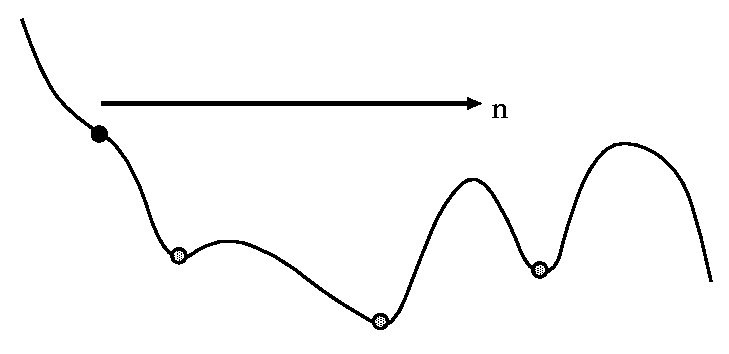
\includegraphics[width=0.6\textwidth]{linemin.eps}
\end{center}
\caption{
Figure for line minimization.
\label{fig:linmin}}
\end{figure}


In the first part of the line minimization routine the minimum is
bracketed, \ie we want a point $\a + s \nhat$ which has a lower
$\chi^2$ value than the points $\a + (s - ds) \nhat$
and $\a + (s + ds) \nhat$, where $ds$ is the step size.

When the line search routine is called, $ds = ds_i$.Here

\begin{eqnarray}
ds_i &=& {0.10 \chi^2 \over ||H||}
\end{eqnarray}

or equal to a value supplied by the user.


Steps with lengths $ds$ are taken along the direction $\nhat$ until
$\chi^2_{n-1} < \chi^2_{n}$, $n=1, \ldots$. If $\chi^2_{n-2} < \chi^2_{n-1}$,
\ie then the line search is restarted from $s=0$ with half the value of $ds$.

In the second part of the routine, a golden search is used to
narrow down the bracket triplet.




\begin{table}[!h]
\caption{
Sub-keywords for \textrm{prop} in table~\ref{tab:kw-sf}
concerning line minimization.
\label{tab:kw-lm-prop}
}
\begin{center}
\begin{tabular}{l|l}
\hline
\hline
\verb+ds_ini+       & Initial step size $ds_i$ when doing line minimization \\
                    & when fitting the properties parameters. \\
\hline
\hline
\end{tabular}
\end{center}
\end{table}


\begin{table}[!h]
\caption{
Sub-keywords for \textrm{pot} in table~\ref{tab:kw-sf}
concerning line minimization.
\label{tab:kw-lm-pot}
}
\begin{center}
\begin{tabular}{l|l}
\hline
\hline
\verb+ds_ini+       & Initial step size $ds_i$ when doing line minimization \\
                    & when fitting the potential parameters. \\
\hline
\hline
\end{tabular}
\end{center}
\end{table}













\subsection{Force calculation preliminaries}

Let the total potential energy of a system consisting of $N$ atoms be

\begin{equation}
V \equiv V(\rr_1, \ldots, \rr_N) = \sum_i V_i,
\end{equation}

where $V_i$ is the energy of atom $i$. The potential can be written
as a sum of $n$-body interactions:

\begin{equation}
V_i = \sum_j V^{(2)}_{ij}(\rr_i, \rr_j)
  + \sum_j \sum_k V^{(3)}_{ijk}(\rr_{ij}, \rr_{ik}, \rr_{jk})
  + \ldots
+ \left( \sum_{i_1} \ldots \sum_{i_M} \right) V^{(M-1)}_{i_1 \ldots i_M} + \ldots
\end{equation}

Here $V_{ij}$ is a pair potential, $V_{ijk}$ a three-body potential, and
$V_{i_1 \ldots i_M}$ is a general $M-1$-body interaction.


How do we calculate the force on any atom, say $v$ ? A fool-prof method is to
calculate the total derivative of the potential with respect to the
position $\rr_v$ of atom $v$:

\begin{eqnarray}
\F_v
  &=& - \nabla_{\rr_v} V \\
  &=& - \sum_{ij} \nabla_{\rr_v} V_{ij} - \sum_{ijk} \nabla_{\rr_v} V_{ijk} - \ldots \\
  &=& - \sum_{i} \nabla_{\rr_v} V_{iv} - \sum_{j} \nabla_{\rr_v} V_{vj} \nonumber \\
  & & - \sum_{ij} \nabla_{\rr_v} V_{ijv}  - \sum_{ik} \nabla_{\rr_v} V_{ivk} - \sum_{jk} \nabla_{\rr_v} V_{vjk} - \ldots \\
  &=& \sum_{i} \F_{iv} + \sum_{j} \F_{vj} \nonumber \\
  & & + \sum_{ij} \F_{ijv} + \sum_{ik} \F_{ivk} + \sum_{jk} \F_{vjk} + \ldots
\end{eqnarray}

Rewriting we have

\begin{eqnarray}
\F_v
  &=& \sum_{i} (\F_{iv} + \F_{vi} ) + \sum_{ij} (\F_{ijv} + \F_{ivj} + \F_{vij}) + \ldots
\label{eq:MD:F:atom}
\end{eqnarray}


\stars


If we have a pair potential, then the energy can be expressed as a function
of the distance $r_{ij}$ between atoms $i$ and $j$:

\begin{equation}
V = \sum_i \sum_j V_{ij}(r_{ij})
\end{equation}

and the total force on atom $v$ is

\begin{eqnarray}
\F_v &=& - \nabla_{\rr_v} \sum_j V_{vj} - \nabla_{\rr_v} \sum_i V_{iv} \\
  & \equiv & \sum_j \F_{v \Leftarrow j} + \sum_i \nabla_{\rr_i} \sum_i V_{iv} \\
  & \equiv & \sum_j \F_{v \Leftarrow j} - \sum_i \F_{i \Leftarrow v} \\
  &=& \sum_j \F_{v \Leftarrow j} + \sum_i \F_{v \Leftarrow i} \\
  &=& 2 \sum_j \F_{v \Leftarrow j},
\end{eqnarray}

where $\F_{v \Leftarrow j}$ is the force on atom $v$ due to interaction
with atom $j$. Here we used

\begin{eqnarray}
\nabla_{\rr_v} f(r_{iv})
  &=& - {\partial f(r_{iv}) \over \partial r_{iv}} {\rr_i - \rr_v \over r_{iv}} \\
  &=& - \nabla_{\rr_i} f(r_{iv}),
\end{eqnarray}



Hence we can use the following alternative method of calculating the force on any atom $v$:

\begin{eqnarray}
\F_v &=& \sum_{j=1, j \neq v}^N \F_{\v \Leftarrow j}, \\
\F_{\v \Leftarrow j} &=& - \sum_j \nabla_{\rr_v} V_{vj} = - {\partial V(r_{vj}) \over \partial r_{vj}} {\rr_v - \rr_j \over r_{vj}}, \\
\F_j &=& \F_j + (- \F_{v \Leftarrow j}), \quad j = 1, \ldots, N, j \neq v.
\end{eqnarray}

In summary: For the force on atom $v$ we use only the $V_{vj}$ term, and get the
contribution from $V_{jv}$ via Newton's third law when we calculate the
force on atom $j$.

\stars

Let's try the same thing with a three-body potential:


\begin{eqnarray}
V &=& \sum_i \sum_j \sum_k V_{ijk}(r_{ij}, r_{ik}, r_{jk}) \\
\F_v &=& \sum_j \sum_k \left(
  {\partial V_{vjk} \over \partial r_{vj}} {\rr_v - \rr_j \over r_{vj}}
+ {\partial V_{vjk} \over \partial r_{vk}} {\rr_v - \rr_k \over r_{vk}} \right) \\
  &=& \sum_j \sum_k \left( \F_{vj} + \F_{vk} \right) \\
\F_j &=& \F_j + (- \F_{v \Leftarrow j}), \\
\F_k &=& \F_k + (- \F_{v \Leftarrow k})
\end{eqnarray}


However, we are now missing terms that does not depend on the distances
$r_{vj}, r_{vk}, r_{jk}$ ! For instance, consider the cosine of the angle
between the bonds $\rr_v - \rr_j$ and $\rr_v - \rr_k$:

\begin{eqnarray}
\cos \theta_{vjk} &=& {(\rr_v - \rr_j) \cdot (\rr_v - \rr_k) \over r_{vj} r_{vk}}
\end{eqnarray}

It is not possible to differentiate this expression with respect to $r_{vj}, r_{vk}, r_{jk}$,
due to the scalar product in the numerator ! In this case we have to use the full
expression in Eq.~(\ref{eq:MD:F:atom}).







\subsection{Pressure calculation}

The pressure is calculated as

\begin{equation}
P = (N k_B T + W/3)/V,
\end{equation}

where $W$ is the virial:

\begin{equation}
W = - 3 V {\partial U \over \partial V}
\end{equation}

See Ref.~\cite{Koster-PRB62-2000,Beardmore-PRB60-1999}.

Writing

\begin{equation}
\rr_k = V^{1/3} \rho_k,
\end{equation}

where $\rho_k$ are dimensionless coordinates independent of the volume, we have

\begin{equation}
{\partial \over \partial V}
= \sum_k {\partial \rr_k \over \partial V} \cdot \nabla_{\rr_k}
= {1 \over 3} V^{-1} \sum_k V^{1/3} \rho_k \cdot \nabla_{\rr_k}
= {1 \over 3} V^{-1} \sum_k \rr_k \cdot \nabla_{\rr_k}
\end{equation}

so that

\begin{eqnarray}
W &=& - \sum_k \rr_k \cdot \nabla_{\rr_k} U
= - \sum_i \sum_{j, j\neq i} \sum_k \nabla_{\rr_k} U^{ij} \cdot \rr_k
\nonumber \\
  &=& \sum_i \sum_{j, j\neq i} \sum_k \F^{ij}_k \cdot \rr_k
\end{eqnarray}

For a pair potential:

\begin{eqnarray}
W &=& \sum_i \sum_{j, j\neq i} \sum_k \F^{ij}_k \cdot \rr_k
= \sum_i \sum_{j, j\neq i} \left( 
\F^{ij}_i \cdot \rr_i + \F^{ij}_j \cdot \rr_j
\right)
\nonumber \\
  &=& \sum_i \sum_{j, j\neq i} \left( 
\F^{ij}_i \cdot \rr_i - \F^{ij}_i \cdot \rr_j
\right)
\nonumber \\
  &=& \sum_i \sum_{j, j\neq i} \F^{ij}_i \cdot \rr_{ij}
\end{eqnarray}

For a many-body potential of the ABOP-form holds that

\begin{eqnarray}
\F^{ij}_i &=& - \sum_{k, k\neq i} \F^{ij}_k
\end{eqnarray}


Note:

\begin{eqnarray}
\sum_i \sum_{j, j\neq i} \sum_{k, k\neq i} \F^{ij}_k \cdot \rr_{ki}
&=&
\sum_i \sum_{j, j\neq i} \sum_{k, k\neq i} \F^{ij}_k \cdot \rr_k
-
\sum_i \sum_{j, j\neq i} \sum_{k, k\neq i} \F^{ij}_k \cdot \rr_i
\\
&=&
\sum_i \sum_{j, j\neq i} \sum_{k, k\neq i} \F^{ij}_k \cdot \rr_k
+
\sum_i \sum_{j, j\neq i} \F^{ij}_i \cdot \rr_i
\\
&=&
\sum_i \sum_{j, j\neq i} \sum_k \F^{ij}_k \cdot \rr_k
\end{eqnarray}

Therefore,

\begin{eqnarray}
W &=& \sum_i \sum_{j, j\neq i} \sum_{k, k\neq i} \F^{ij}_k \cdot \rr_{ki}
\end{eqnarray}









\subsection{Lennard-Jones potential}

The 6-12 Lennard-Jones potential gives the total energy of a dimer
with bond length $r_{ij}$  as

\begin{equation}
E_{dimer} = 4 \eps \left[
  \left({\sigma \over r_{ij}}\right)^{12}
- \left({\sigma \over r_{ij}}\right)^{6}
\right]
\label{eq:LJ}
\end{equation}

Here

\begin{equation}
r_{ij} = |\rr_i - \rr_j| = r_{ji}
\end{equation}



At equilibrium $E_{dimer} = -\eps$, making the energy per atom, \ie
the cohesive energy $E_c$, $-\eps/2$.
By definition,

\begin{equation}
E_c = {1 \over N} \sum_i \sum_j E_{ij},
\end{equation}

Here $E_{ij}$ is the energy contribution to atom $i$
due to neighbor $j$. Putting

\begin{equation}
E_{ij} = A E_{dimer}
\end{equation}

we get from the cohesive energy equation that

\begin{equation}
-\eps = A (-2\eps)
\end{equation}

so that $A=1/2$. This means that

\begin{equation}
E_{ij} = 2 \eps \left[
  \left({\sigma \over r_{ij}}\right)^{12}
- \left({\sigma \over r_{ij}}\right)^{6}
\right]
\end{equation}

in the formula

\begin{equation}
E = \sum_{i=1}^N \sum_{j, j\neq i}^N E_{ij}
\end{equation}

for the energy of an atom system.

The force on atom $i$ is

\begin{equation}
\F_{ij} = 
- 12 \eps \left[
 2 \left( {\sigma \over r_{ij}} \right)^{12}
-  \left( {\sigma \over r_{ij}} \right)^6
\right]
{\rr_i - \rr_j \over r^2_{ij}}
\end{equation}









\subsection{Morse potential}

The Morse potential gives the total energy of a dimer as

\begin{equation}
E_{dimer} = D \left[
e^{-2\beta(r_{ij}-r_0)} - 2 e^{-\beta(r_{ij}-r_0)]}
\right]
\label{eq:morse}
\end{equation}

At equilbrium, $r_{ij} = r_0$,

\begin{equation}
E_{dimer} = -D
\end{equation}

Cohesive energy is then $E_c = -D/2$. As above, we obtain

\begin{equation}
E_{ij}
= {1 \over 2} D \left[
e^{-2\beta(r_{ij}-r_0)} - 2 e^{-\beta(r_{ij}-r_0)]}
\right]
\end{equation}

We now have

\begin{equation}
\F_{ij}
= - D \beta  \left[
e^{-2\beta(r_{ij}-r_0)} - e^{-\beta(r_{ij}-r_0)]}
\right]
{\rr_i - \rr_j \over r_{ij}}
\end{equation}



\stars

Some essential derivatives are:

\begin{eqnarray}
\nabla_i V_{R,ij} &=& - {D_0 \beta \sqrt{2S} \over S-1} 
\exp\left[ - \beta \sqrt{2S} (r_{ij} -r_{0,ij}) \right] {\rr_i - \rr_j \over r_{ij}}
\\
\nabla_i V_{A,ij} &=& - {S D_0 \beta \sqrt{2/S} \over S-1}
\exp\left[ - \beta \sqrt{2/S} (r_{ij} -r_{0,ij}) \right] {\rr_i - \rr_j \over r_{ij}}
\\
\nabla_i f_{C,ij} &=& {\rr_i - \rr_j \over r_{ij}}
\left\{
\begin{array}{ll}
0,                   & r \leq R - D, \\
-{\pi \over 4 D} \cos \left( {\pi \over 2} {r_{ij} - R \over D} \right), & |R - r_{ij}| < D  \\
0,                   & r \geq R + D
\end{array}
\right.
\\
\nabla_i b_{ij}
 &=& - {1 \over 2 (1 + \chi_{ij})^{3/2}} \nabla_{\rr_i} \chi_{ij} \\
\nabla_i \chi_{ij}
  &=&
  \sum_{k, k \neq i, k \neq j} (\nabla_{\rr_i} f_{C,ik}) g_{ijk} \omega_{ijk} \exp\left[
  \alpha_{ijk}(r_{ij} - r_{ik}) \right] \nonumber \\
  & &
+ \sum_{k, k \neq i, k \neq j} f_{C,ik} (\nabla_{\rr_i} g_{ijk}) \omega_{ijk} \exp\left[
  \alpha_{ijk}(r_{ij} - r_{ik}) \right]  \nonumber \\
  & &
+ \sum_{k, k \neq i, k \neq j} f_{C,ik} g_{ijk} \omega_{ijk} \nabla_{\rr_i} \exp\left[
  \alpha_{ijk}(r_{ij} - r_{ik}) \right]
\\
\nabla_i g_{ijk}
  &=& \gamma {c^2 \over (d^2 + (h + \cos \theta_{ijk})^2)^2} 2 (h + \cos \theta_{ijk})
\nabla_i \cos \theta_{ijk}
\end{eqnarray}

and

\begin{eqnarray}
\nabla_i \cos \theta_{ijk}
  &=& \nabla_i { (\rr_j - \rr_i) \cdot (\rr_k - \rr_i) \over r_{ij} r_{ik}} \\
  &=&
\nabla_i { \rr_j \cdot \rr_k - \rr_j \cdot \rr_i - \rr_i \cdot \rr_k + r_i^2
\over r_{ij} r_{ik} } \\
  &=&
{1 \over r_{ij} r_{ik} }
( - \rr_j - \rr_k + 2 \rr_i )
\nonumber \\
  & &
- {\cos \theta_{ijk} \over r_{ij}} {\rr_i - \rr_j \over r_{ij}}
- {\cos \theta_{ijk} \over r_{ik}} {\rr_i - \rr_k \over r_{ik}}
\nonumber \\
  &=&
  (\rr_i - \rr_j) \left[
  {1 \over r_{ij} r_{ik} }
- {\cos \theta_{ijk} \over r^2_{ij}}
\right]
\nonumber \\
  & &
 +(\rr_i - \rr_k) \left[
  {1 \over r_{ij} r_{ik} }
- {\cos \theta_{ijk} \over r^2_{ik}}
\right]
\end{eqnarray}

and also

\begin{eqnarray}
  & & \nabla_{\rr_i} \exp\left[ \alpha_{ijk}(r_{ij} - r_{ik}) \right] \\
  &=&
{ \rr_i - \rr_j \over r_{ij}} \alpha_{ijk} \exp\left[ \alpha_{ijk}(r_{ij} - r_{ik}) \right]
-
{ \rr_i - \rr_k \over r_{ik}} \alpha_{ijk} \exp\left[ \alpha_{ijk}(r_{ij} - r_{ik}) \right]
\end{eqnarray}




With

\begin{equation}
V = {1 \over 2} \sum_i \sum_{j} f_{C,ij} \left( V_{R,ij} - b_{ij} V_{A,ij} \right)
\end{equation}

the force on atom $v$ is

\begin{eqnarray}
\F_v &=&
      - {1 \over 2} \sum_j (\nabla_v f_{C,vj}) \left( V_{R,vj} - b_{vj} V_{A,vj} \right)
\nonumber \\
  & & - {1 \over 2} \sum_j (\nabla_v f_{C,jv}) \left( V_{R,jv} - b_{jv} V_{A,jv} \right)
\nonumber \\
  & & - {1 \over 2} \sum_j f_{C,vj} \left( (\nabla_v V_{R,vj}) - b_{vj} (\nabla_v V_{A,vj})
- (\nabla_v b_{vj}) V_{A,vj} \right)
\nonumber \\
  & & - {1 \over 2} \sum_j f_{C,jv} \left( (\nabla_v V_{R,jv}) - b_{jv} (\nabla_v V_{A,jv})
- (\nabla_v b_{jv}) V_{A,jv} \right)
\nonumber \\
  & & + {1 \over 2} \sum_i \sum_j f_{C,ij} (\nabla_v b_{ij}) V_{A,ij}
\\
  &=& - {1 \over 2} \sum_j (\nabla_v f_{C,vj}) \left( V_{R,vj} - b_{vj} V_{A,vj} \right)
\nonumber \\
  & & - {1 \over 2} \sum_j (\nabla_v f_{C,jv}) \left( V_{R,jv} - b_{jv} V_{A,jv} \right)
\nonumber \\
  & & - {1 \over 2} \sum_j f_{C,vj} \left( (\nabla_v V_{R,vj}) - b_{vj} (\nabla_v V_{A,vj})\right)
\nonumber \\
  & & - {1 \over 2} \sum_j f_{C,jv} \left( (\nabla_v V_{R,jv}) - b_{jv} (\nabla_v V_{A,jv})\right)
\nonumber \\
  & & + {1 \over 2} \sum_j (\nabla_v b_{vj}) V_{A,vj}
\nonumber \\
  & & + {1 \over 2} \sum_j (\nabla_v b_{jv}) V_{A,jv}
\nonumber \\
  & & + {1 \over 2} \sum_i \sum_j f_{C,ij} (\nabla_v b_{ij}) V_{A,ij}
\end{eqnarray}

Notice the last term in this expression. It is crucial.
Notice also that it is added only when $i \neq v \neq j$, \ie for atom $k$ in the sum for $b_{ij}$.


\stars


\begin{eqnarray}
W &=& \sum_i \sum_{j, j\neq i} \sum_{k, k\neq i} \F^{ij}_k \cdot \rr_{ki},
\end{eqnarray}

where

\begin{eqnarray}
\sum_{k, k\neq i} \F^{ij}_k \cdot \rr_{ki}
  &=&
- \nabla_{\rr_j} \left[ f_c(r_{ij}) V_R(r_{ij}) - b_{ij} f_c(r_{ij}) V_A(r_{ij}) \right] \cdot \rr_{ji}
\nonumber \\
  & &
+ f_c(r_{ij}) V_A(r_{ij}) \sum_{k, k\neq i,j} \nabla_{\rr_k} b_{ij} \cdot \rr_{ki}
\end{eqnarray}

Note: Earlier we had derivatives with respect to $\rr_{i}$. The current derivatives of $b_{ij}$
will be different !!!


\begin{eqnarray}
\nabla_j \chi_{ij}
  &=&
  \sum_{k, k \neq i, k \neq j} f_{C,ik} (\nabla_{\rr_j} g_{ijk}) \omega_{ijk} \exp\left[
  \alpha_{ijk}(r_{ij} - r_{ik}) \right]  \nonumber \\
  & &
+ \sum_{k, k \neq i, k \neq j} f_{C,ik} g_{ijk} \omega_{ijk} \nabla_{\rr_j} \exp\left[
  \alpha_{ijk}(r_{ij} - r_{ik}) \right]
\end{eqnarray}


\begin{eqnarray}
\nabla_j \cos \theta_{ijk}
  &=& \nabla_j { (\rr_j - \rr_i) \cdot (\rr_k - \rr_i) \over r_{ij} r_{ik}} \\
  &=&
\nabla_j { \rr_j \cdot \rr_k - \rr_j \cdot \rr_i - \rr_i \cdot \rr_k + r_i^2
\over r_{ij} r_{ik} } \\
  &=&
{- \rr_{ik} \over r_{ij} r_{ik} }
- 
{ \rr_{ij} \cdot \rr_{ik} \over r_{ij}^2 r_{ik}} \left( -{\rr_{ij} \over r_{ij}} \right) \\
  &=&
{- \rr_{ik} \over r_{ij} r_{ik} }
- 
{ \cos \theta_{ijk} \over r_{ij}} \left( -{\rr_{ij} \over r_{ij}} \right) \\
  &=&
{1 \over r_{ij} r_{ik}}
\left[
- \rr_{ik} + \cos \theta_{ijk} r_{ik} {\rr_{ij} \over r_{ij}}
\right]
\\
  &=& 
{1 \over r_{ij}}
\left[
- {\rr_{ik} \over r_{ik}}
+ \cos \theta_{ijk} {\rr_{ij} \over r_{ij}}
\right]
\end{eqnarray}



\begin{eqnarray}
\nabla_k \cos \theta_{ijk}
  &=& \nabla_k { (\rr_j - \rr_i) \cdot (\rr_k - \rr_i) \over r_{ij} r_{ik}} \\
  &=&
\nabla_k { \rr_j \cdot \rr_k - \rr_j \cdot \rr_i - \rr_i \cdot \rr_k + r_i^2
\over r_{ij} r_{ik} } \\
  &=&
{\rr_j - \rr_i \over r_{ij} r_{ik}}
+
{\rr_{ji} \cdot \rr_{ki} \over r_{ik}^2 r_{ij}} {\rr_{ik} \over r_{ik}}
\\
  &=&
{- \rr_{ij} \over r_{ij} r_{ik}}
+
\cos \theta_{ijk} {\rr_{ik} \over r_{ik}^2}
\end{eqnarray}



When \eg only $d$-band contributes to the energy, then the force on atom $v$ is

\begin{eqnarray}
\F_v
  &=&
- {1 \over 2} \nabla_v \sum_i \sum_j V_{2,ij}
- \nabla_v \sum_i F_{d,i}(\rho^a_{i})
\nonumber \\
  &=&
- {1 \over 2} \nabla_v \sum_j V_{2,vj}
- \nabla_v \sum_i F_{d,i}(\sum_j \rho_{ij}(r_{ij})) \nonumber \\
  &=&
- {1 \over 2} \nabla_v \sum_j V_{2,vj}
\nonumber \\
  & &
- {\partial F_{d,v}(\rho^a_v) \over \partial \rho^a_v} \sum_j {\partial \rho^a_v \over \partial r_{vj}} {\rr_v - \rr_j \over r_{vj}}
\nonumber \\
  & &
+ \sum_j  {\partial F_{d,j}(\rho^a_j) \over \partial \rho^a_j} {\partial \rho^a_j \over \partial r_{jv}} {\rr_j - \rr_v \over r_{jv}}
\nonumber \\
  &=&
- {1 \over 2} \nabla_v \sum_j V_{2,vj} \nonumber \\
  & &
- \sum_j  \left(
  {\partial F_{d,v}(\rho^a_v) \over \partial \rho^a_v}
+ {\partial F_{d,j}(\rho^a_j) \over \partial \rho^a_j}
\right)
{\partial \rho^a_j \over \partial r_{vj     }} {\rr_v - \rr_j \over r_{vj}}
\end{eqnarray}

